%----------------------------------------------------------------------------------------
%	PACKAGES AND OTHER DOCUMENT CONFIGURATIONS
%----------------------------------------------------------------------------------------

	\documentclass[a4paper, 11pt, oneside]{book}

	\usepackage[sc]{mathpazo} % Use the Palatino font
	\usepackage[utf8]{inputenc}
	\usepackage[spanish, es-tabla]{babel}
	\decimalpoint
	
	\usepackage{lipsum}
	\usepackage{graphicx}
	\usepackage[T1]{fontenc} % Use 8-bit encoding that has 256 glyphs
	\linespread{1.15} % Line spacing - Palatino needs more space between lines
	%\usepackage{microtype} % Slightly tweak font spacing for aesthetics
	%
	\usepackage[hmarginratio=1:1,left=20mm, top=22mm]{geometry} % Document margins
	%\usepackage{multicol} % Used for the two-column layout of the document
	\usepackage[hang, small,labelfont=bf,up,textfont=it,up]{caption} % Custom captions under/above floats in tables or figures
	\usepackage{mathtools}
	%\usepackage{booktabs} % Horizontal rules in tables
	\usepackage{float} % Required for tables and figures in the multi-column environment - they need to be placed in specific locations with the [H] (e.g. \begin{table}[H])
	\usepackage{hyperref} % For hyperlinks in the PDF
	\usepackage{appendix}
	\usepackage{subcaption}
	%\usepackage{wrapfig}
	%%\usepackage[]{mcode} % For embebing matlab code
	%\usepackage[makeroom]{cancel}
	%
	%%\usepackage{lettrine} % The lettrine is the first enlarged letter at the beginning of the text
	%\usepackage{paralist} % Used for the compactitem environment which makes bullet points with less space between them
	%
	%\usepackage{abstract} % Allows abstract customization
	%\renewcommand{\abstractnamefont}{\normalfont\bfseries} % Set the "Abstract" text to bold
	%\renewcommand{\abstracttextfont}{\normalfont\small\itshape} % Set the abstract itself to small italic text
	%%%
	%\usepackage{titlesec} % Allows customization of titles
	%%\renewcommand\thesection{\Roman{section}} % Roman numerals for the sections
	%%\renewcommand\thesubsection{\Roman{subsection}} % Roman numerals for subsections
	%\titleformat{\section}[block]{\large\scshape\centering}{\thesection.}{1em}{} % Change the look of the section titles
	%\titleformat{\subsection}[block]{\large\centering}{\thesubsection.}{1em}{} % Change the look of the section titles
	%
	%\usepackage{fancyhdr} % Headers and footers
	%\pagestyle{fancy} % All pages have headers and footers
	%\fancyhead{} % Blank out the default header
	%\fancyfoot{} % Blank out the default footer
	%\fancyhead[C]{Titulo Corto% based on TRACS 
	%\hspace{4pt} $\bullet$ \hspace{4pt} MES ANO } % Custom header text
	%\fancyfoot[RO,LE]{\thepage} % Custom footer text
	%
	\usepackage{cite}
	\usepackage{listings}
	\usepackage{color}

	\graphicspath{{../Graphics/}}
	%
	%\DeclareGraphicsExtensions{.pdf,.png,.jpg} % Graphics type

	\newcommand{\ibias}{$I_{Bias}$}
	\newcommand{\chirp}{\textit{Chirp}}
	\newcommand{\I}{corriente de inyecci\'on $I(t)$}
	\newcommand{\n}{densidad de portadores de carga $N(t)$}
	\newcommand{\s}{densidad de fotones $S(t)$}
	\newcommand{\fase}{fase \'optica $\Phi(t)$}
%----------------------------------------------------------------------------------------
%	   METADATA
%----------------------------------------------------------------------------------------

	%\title{
	%	\selectfont\textbf{TITULO}% Article title
	%}
%
	%\author{
	%	\textsc{Jaime Diez Gonzalez-Pardo}\\
	%	%\thanks{A thank you or further information}\\ % Your name
	%	\fontsize{28pt}{10pt} Universidad de Cantabria \\ % Your institution
	%	%\thanks{A thank you or further information}\\[2mm] % Your name
	%	\normalsize gsdfgdfgdfgatura \\ 
	%	\normalsize{Compañeros:} \textsc{NOMBRE COMPANEROS }\\
	%	%\vspace{5mm}
	%}
%
	%\date{\today}

%----------------------------------------------------------------------------------------
%      · DOCUMENT
%----------------------------------------------------------------------------------------

	\begin{document}

		\begin{titlepage} 

			\newcommand{\HRule}{\rule{\linewidth}{0.5mm}} 
			
			\center % Centre everything on the page
			
			%------------------------------------------------
			%	Headings
			%------------------------------------------------
			
				%------------------------------------------------
				%	Logo
				%------------------------------------------------
				
					\begin{figure}[H]
						\centering
						
\includegraphics[scale=0.6]{download.png}
					\end{figure}

					\textsc{\LARGE Facultad de Ciencias}\\[1.5cm] 
			
			
			%------------------------------------------------
			%	Title
			%------------------------------------------------
			
				\HRule\\[0.4cm]
				
				{\huge\bfseries Simulación de peines de frecuencia óptica generados por láseres de semiconductor}\\[0.8cm] % Title of your document

				{\huge Simulation of optical frequecy comb generate by semiconductor lasers}\\[0.4cm] % Title of your document
				
				\HRule\\[1.5cm]

				{\Large Trabajo de Fin de Grado para acceder al}\\[0.4cm]

				{\LARGE\bfseries Grado en Física}\\[3cm]
			
			%------------------------------------------------
			%	Author(s)
			%------------------------------------------------
			
				\begin{flushright}
					\large
					\textit{Autor}\\
					Jaime \textsc{DÍEZ GONZÁLEZ-PARDO} \\ % Your name
					\large
					\textit{Director}\\
					Dr. Á.A. \textsc{VALLE GUTIERREZ} % Supervisor's name
				\end{flushright}
			
			%------------------------------------------------
			%	Date
			%------------------------------------------------
			
				\vfill\vfill\vfill % Position the date 3/4 down the remaining page
				
				{\large\today} % Date, change the \today to a set date if you want to be precise
				
			%----------------------------------------------------------------------------------------
			
				\vfill % Push the date up 1/4 of the remaining page
		
		\end{titlepage}

		%\thispagestyle{fancy} % All pages have headers and footers

		\tableofcontents

		\listoffigures

		%----------------------------------------------------------------------------------------
		%	  ARTICLE CONTENTS
		%----------------------------------------------------------------------------------------

			\addtocontents{toc}{\vspace{0.1cm}}
			\chapter{Introducción} % Scope of the project = rad effects + minimization
				\label{Intr}

				%\input{}

				\addtocontents{toc}{\vspace{0.1cm}}
				\section{Láseres de Semiconductor}
					\label{Intr:LsrSmcdtr}
					
					%\input{}

				\addtocontents{toc}{\vspace{0.1cm}}
				\section{Procesos Estocásticos}
					\label{Intr:PrcsEstcs}
					
					%\input{}

				\addtocontents{toc}{\vspace{0.1cm}}
				\section{Dinámica No Lineal}
					\label{Intr:NonLnr}
					
					%\input{}
%
				\addtocontents{toc}{\vspace{0.1cm}}
				\section{Peines de Frecuencia Óptica}
					\label{Intr:OFC}
					
					
Que son, caracteristicas principales y como se generan,...

	\subsection{\textit{Gain-Switching}}

		hola que tal todos

	\subsection{Inyección Ópticar}

		adios a todos 

	\subsection{Aplicaciones}




				\addtocontents{toc}{\vspace{0.1cm}}
				\section{Objetivo del Estudio}
					\label{Intr:Obj}
					
					%\input{}
				
			\addtocontents{toc}{\vspace{0.1cm}}
			\chapter{Modelo Computacional}
				\label{Mdl}

				\addtocontents{toc}{\vspace{0.1cm}}
				\section{RoF}
					\label{Mdl:RoF}
				
					%\input{}

				\addtocontents{toc}{\vspace{0.1cm}}
				\section{Código de la Simulación}
					\label{Mdl:Code}
				
					\definecolor{gray97}{gray}{.97}
\definecolor{gray75}{gray}{.75}
\definecolor{gray45}{gray}{.45}

\lstset{ frame=Ltb,
	framerule=0pt,
	aboveskip=0.1cm,
	framextopmargin=3pt,
	framexbottommargin=3pt,
	framexleftmargin=0.4cm,
	framesep=0pt,
	rulesep=.4pt,
	backgroundcolor=\color{gray97},
	rulesepcolor=\color{black},
	%
	stringstyle=\ttfamily,
	showstringspaces = false,
	basicstyle=\small\ttfamily,
	commentstyle=\color{gray45},
	keywordstyle=\bfseries,
	%
	numbers=left,
	numbersep=15pt,
	numberstyle=\tiny,
	numberfirstline = false,
	breaklines=true,
}

\lstdefinestyle{Python}
{basicstyle=\scriptsize\bf\ttfamily,
language=python,
}

\centering\small
\vspace{0.4cm} +- - - - - - - - - - - - - 18 l\'ineas - - - - - - - - - - - - -+
\lstinputlisting[style=Python, firstline=19, lastline=26, firstnumber=19]{../src/simulation.py}
\vspace{-0.4cm} +- - - - - - - - - - - - - 18 l\'ineas - - - - - - - - - - - - -+
\lstinputlisting[style=Python, firstline=44, lastline=53, firstnumber=44]{../src/simulation.py}

\vspace{-0.4cm} +- - - - - - - - - - - - - 24 l\'ineas - - - - - - - - - - - - -+
\lstinputlisting[style=Python, firstline=77, lastline=81, firstnumber=77]{../src/simulation.py}

\vspace{-0.4cm} +- - - - - - - - - - - - - 15 l\'ineas - - - - - - - - - - - - -+
\lstinputlisting[style=Python, firstline=96, lastline=96, firstnumber=96]{../src/simulation.py}

\vspace{-0.4cm} +- - - - - - - - - - - - - 20 l\'ineas - - - - - - - - - - - - -+
\newpage
\lstinputlisting[style=Python, firstline=116, lastline=155, firstnumber=116]{../src/simulation.py}

\vspace{-0.4cm} +- - - - - - - - - - - - - 10 l\'ineas - - - - - - - - - - - - -+
\newpage
\lstinputlisting[style=Python, firstline=165, lastline=192, firstnumber=165]{../src/simulation.py}

\vspace{-0.4cm} +- - - - - - - - - - - - - 10 l\'ineas - - - - - - - - - - - - -+
\lstinputlisting[style=Python, firstline=202, lastline=206, firstnumber=202]{../src/simulation.py}

\vspace{-0.4cm} +- - - - - - - - - - - - -  6 l\'ineas - - - - - - - - - - - - -+
\lstinputlisting[style=Python, firstline=212, lastline=220, firstnumber=212]{../src/simulation.py}

\vspace{-0.4cm} +- - - - - - - - - - - - - 39 l\'ineas - - - - - - - - - - - - -+
%\lstinputlisting[style=Python, firstline=96, lastline=220, firstnumber=100]{../src/simulation.py}

				
			\addtocontents{toc}{\vspace{0.1cm}}
			\chapter{Láser en solitario}

				\graphicspath{{../Graphics/Cpt1-Charactz/}}

\newcommand{\cw}{corriente continua}

Antes de abordar el estudio de la dinámica no lineal del láser de semiconductor de modo discreto se ha realizado la simulación del láser en solitario, sin inyección de luz del láser esclavo ($P_{Iny} = 0$). Se han realizado simulaciones para el láser tanto en \cw\ (CW de sus siglas en inglés), como en Gain-Switching, comparando los resultados con los obtenidos experimentalmente en condiciones similares \cite{Chaves19}.

	\addtocontents{toc}{\vspace{0.1cm}}
	\section{Láser en \cw}
		
		
Para poder realizar las simulaciones en \cw\ se ha trabajado con una corriente de inyección constante e igual a la corriente de polarización ($I(t) = I_{Bias}$), tomando $V_{RF} = 0$.

HABLAR DE QUE EN CONTINUA SE TIENE QUE $\frac{\mathrm{d} N}{\mathrm{d} t} = \frac{\mathrm{d} S}{\mathrm{d} t} = \frac{\mathrm{d} \Phi}{\mathrm{d} t} = 0$

\addtocontents{toc}{\vspace{0.1cm}}
\subsection{Espectros de emisión}

	Tal y como se vio en la secci\'on \ref{Intr:LsrSmcdtr}, pequeñas variaciones en la corriente de inyección del láser producen desplazamientos de la línea de emisión del láser en el espectro de frecuencias. Por ello es importante conocer el valor de la longitud de onda del pico de emisión del láser en solitario en función de la corriente de polarización \ibias, de cara a realizar el estudio de la inyección de luz.

	En la Figura \ref{Img:spectrosCW} se muestran las densidades espectrales de potencia del l\'aser a diferentes corrientes de polarización, comparando los datos obtenidos mediante la simulaci\'on del l\'aser(Figura \ref{Img:spectrosCW:sim}), con los obtenidos experimentalmente(Figura \ref{Img:spectrosCW:exp}).

		% Img:spectrosCW {Img:spectrosCW:sim, Img:spectrosCW:exp}
		\begin{figure}[H]
			\centering
			\begin{subfigure}{0.45\textwidth}
				\centering
				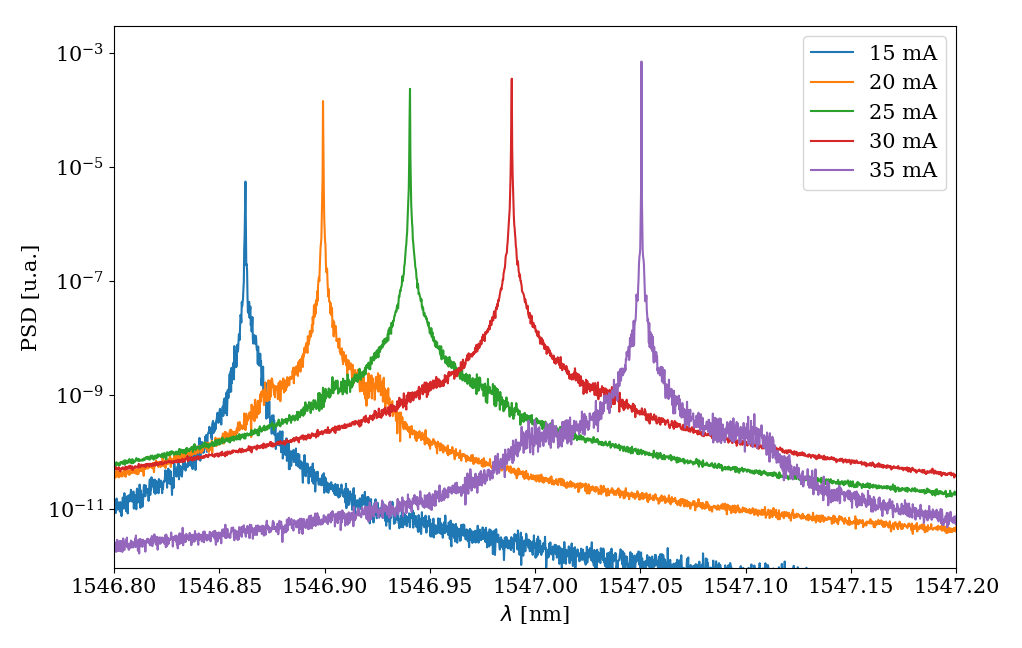
\includegraphics[width=1.0\linewidth, height=6cm]{Espectros.png}
				\caption{\label{Img:spectrosCW:sim}Espectros ópticos obtenidos mediante simulación.}
			\end{subfigure}
			\begin{subfigure}{0.45\textwidth}
				\centering
				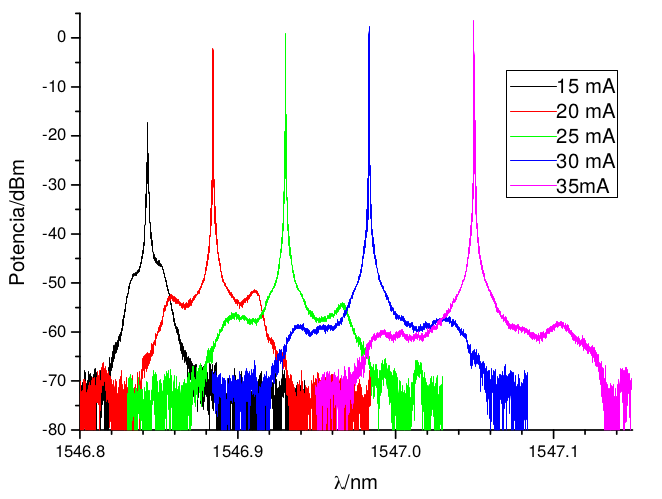
\includegraphics[width=1.0\linewidth, height=6cm]{../Chaves/OFC-GS/espectros_continua.png}
				\caption{\label{Img:spectrosCW:exp}Espectros ópticos obtenidos experimentalmente.}	
			\end{subfigure}
			\caption{\label{Img:spectrosCW}Espectros ópticos del DML para diferentes corrientes de polarización \ibias obtenidos mediante simulación (izquierda \ref{Img:spectrosCW:sim}) y mediante experimento (derecha, \ref{Img:spectrosCW:exp}).}
		\end{figure}

		Comparando los espectros obtenidos mediante simulación con los obtenidos esperimentalmente se observa un gran parecido en la forma, observando una forma m\'as puntiaguda y estrecha en los espectros con corriente $I_{Bias}= 15$ mA para ambas gr\'aficas. Adem\'as, la simulación permite observar los picos propios de las oscilaciones de relajaci\'on del l\'aser que se observan en el experimento.

		Adem\'as, a partir de los espectros de la Figura \ref{Img:spectrosCW} se pueden obtener las longitudes de onda de los picos de emisión en funci'on de la corriente \ibias. En la Tabla \ref{tab:lambdas} se muestran los valores de las longitudes de onda $lambda$ obtenidas de los espectros de la Figura \ref{Img:spectrosCW} tanto para la simulaci\'on como para el experimento.

		% tab:lambdas
		\begin{table}[H]
			\centering
			\begin{tabular}{c c c}
				\hline
				\ibias & $\lambda_{sim}$ & $\lambda_{exp}$ \\\hline 
				15 & 1546.86 & 1546.84 \\
				20 & 1546.90 & 1546.88 \\
				25 & 1546.94 & 1546.93 \\
				30 & 1546.99 & 1546.98 \\
				35 & 1547.05 & 1547.05 \\\hline
			\end{tabular}
			\caption{\label{tab:lambdas}Longitud de onda de las lineas de emisión del DML en función de la \ibias obtenidas de la figura \ref{Img:spectrosCW}. Se muestran los valores experimentales $\lambda_{exp}$ obtenidos de la gráfica \ref{Img:spectrosCW:exp} con un error de $\delta\lambda_{exp} = 0.02$, y los valores obtenidos de la simulación de la gráfica \ref{Img:spectrosCW:sim}.}
		\end{table}

	Los valores de las longitudes de onda que se muestran en la Tabla \ref{tab:lambdas} muestran una gran similitud entre los valores experimentales y los obtenidos mediante simulación, obteniendo una discrepancia m\'axima de $0.02$ nm. De esta forma, la gran concordancia entre los valores de $\lambda$ experimentales y los obtenidos a partir de la simulaci\'on, junto con la gran similitud en la forma de los espectros, muestra la capacidad de la simulaci\'on de reproducir computacionalmente los resultados obtenidos experimentalmente en el laboratorio.

	Para el estudio de la inyecci'on de luz se trabajar\'a con una corriente $I_{Bias} = 35$ mA. Por tanto, la Tabla \ref{tab:lambdas} permite obtener su longitud de onda de emisi\'on de $\lambda = 1547.05$ nm, siendo adem\'as la misma que la obtenida en el experimento.

\addtocontents{toc}{\vspace{0.1cm}}
\subsection{Oscilaciones de Relajaci\'on}

	Para que el l\'aser comience a emitir se ha de cumplir que la emisi\'on estimulada domine frente a la emisi\'on espont\'anea. Esto se produce cuando la densidad de portadores de carga en la regi\'on activa supera un valor umbral, $N_{th}$, a partir del cu\'al el l\'aser comienza a emitir fotones. Si la inyecci\'in de corriente que se le aplica al l\'aser es constante (\cw), la densidad de portadores de carga tender\'a a estabilizarse en $N_{th}$. De el mismo modo, la densidad de fotones y el chirp se estabilizar\'an para valores $S_{th}$ y $\Phi_{th}$.

	No obstante, si se parte de unas condiciones iniciales del l\'aser con valores $N(t=0) < N_{th}$, ser\'a necesario que transcurra un cierto tiempo hasta que el l\'aser alcance el equilibrio y se estabilice. A este tiempo se le denomina transitorio.

	Cabe destacar que, tal y como se coment\'o en el apartado \ref{Mdl:Code:Trans}, para la simulación se ha trabajado con un tiempo de transitorio $t_{trans} = 1.2$ ns, en el cu\'al se ha operado con la raiz cuadrada del m\'odulo de $S$ en los t\'erminos de ruido para evitar resultados complejos, despeciando dicho intervalo en el estudio de los espectros. Sin embargo, en este apartado se estudiar\'an las ecuaciones de balance en el transitorio para corrinte continua. El trabajar con una corriente continua mayor que la corriente umbral permite disminuir el intervalo de tiempo en el que se operar\'a con $\sqrt{|S|}$ hasta los 0.2 ns, pudiendo realizar un estudio m\'as riguroso de las ecuaciones de balance en el transitorio.

	Se considerar\'a una intensidad de corriente $I(t)$ funci\'on escal\'on con $I(t>0) = I_{Bias}$. En la ecuaci\'on \ref{eq:transient} se muestra la funci\'on escal\'on $I(t)$ utilizada as\'i como las condiciones iniciales para la densidad de portadores de carga $N(0)$, la densidad de fotones $S(0)$ y de la fase \'optica $\Phi(0)$.

		%eq:transient
		\begin{equation}
			\begin{matrix}
					I(t) = \left\{\begin{matrix}
									0 & t \leq 0\\ 
									I_{Bias} = 30 \textrm{mA} & t > 0
							\end{matrix}\right.
					& & & & & & 
					\begin{matrix}
						N(0) = N_{tr} \\ S(0) = 10^{15} \textrm{m}^{-3}\\ \Phi(0) = 0
					\end{matrix}
				\end{matrix}
			\label{eq:transient}
		\end{equation}

	En la Figura \ref{Img:transitorio} se muestra la evoluci\'on temporal de la \I\ junto con los valores obtenidos en la simulaci\'on para la \n\, la \s\ y la \fase\ para el transitorio $t_{trans} = 1.2$ ns.

		% Img:transitorio
		\begin{figure}[H]
			\centering
			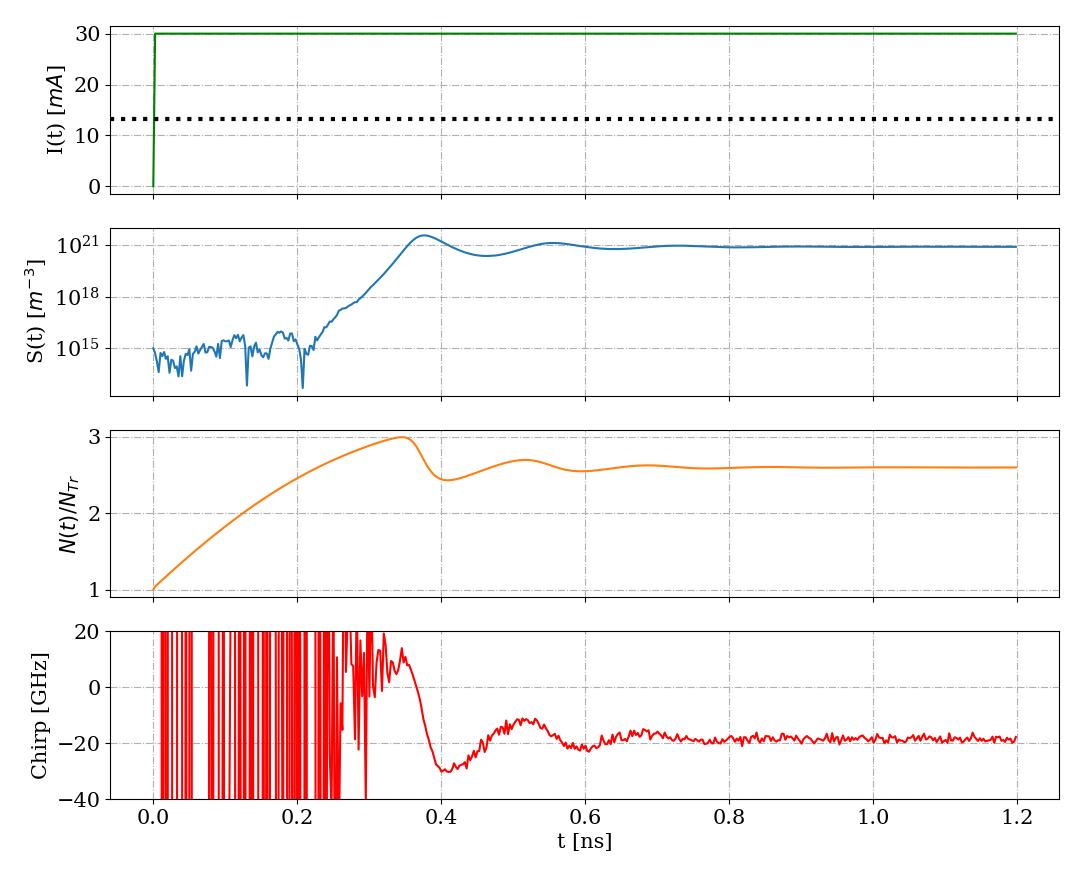
\includegraphics[width=0.7\linewidth]{transitorio.png}
			\caption{\label{Img:transitorio}Evoluci\'on temporal de la \I, la \s, la \n\ y del \chirp\ durante el transitorio. Para la \I\ se ha marcado la corriente umbral del l\'aser $I_{th} = 14.8$ mA con una l\'inea horizontal discontinua.}	
		\end{figure}
		
		Se observan en las evoluciones temporales de \n, \s\ y \fase\ de la Figura \ref{Img:transitorio} tres regiones diferentes en funci\'on del comportamiento de las tres magnitudes: $i$) Una vez que la corriente inyectada supera la corriente umbral $I_{th}$ (en $t=0$) la \n\ comienza a aumentar. No obstante, el valor de $N(t)$ se mantiene inferior a $N_{th}$ por lo que no se produce emisión estimulada, y as\'i, la densidad de fotones no aumenta y toma valores aleatorios, debido a la emisi\'on espont\'anea, alrededor de $S(0)$. Esto tambi\'en se puede observar en el comportamiento tambi\'en aleatorio del \chirp. $ii$) La \n\ continua aumentando alcanzando el valor umbral $N_{th}$ en $t = 0.23$ ns. En este punto la densidad de fotones comienza a aumentar debido a la emisi\'on estimulada producida al superar $N_{th}$. Sin embargo, al encontrarse $S(t)$ por debajo de $S_{th}$, $N(t)$ continua creciendo tomando valores por encima $N_{th}$ hasta que $S(t)$ alcanza el valor de $S_{th}$, en $t \approx 0.37$ ns. Al alcanzar $S(t)$ el valor de $S_{th}$, comienza a dominar la emisi\'on estimulada frente a la emisi\'on espont\'anea. Al alcanzar el valor $S_{th}$ la emisi\'on estimulada domina frente a la emisi\'on espont\'anea, como se puede observar el \chirp, y la densidad de portadores de carga comienza a disminuir, alcanzando la \n\ y \chirp\ un m\'aximo. La densidad de fotones contin\'ua aumentando y la densidad de portadores de carga disminuyendo, llegando nuevamente a tomar valores por debajo de $N_{th}$. Debido a \'esto $S(t)$ alcanza un m\'aximo cuando $N(t) = N_{th}$ y comienza a disminuir, volviendo a tomar valores inferiores a $S_{th}$ y as\'i, volviendo a aumentar $N(t)$. Estas oscilaciones entorno a los valores umbrales continuan, disminuyendo su amplitud, realizando un comportamiento anarm\'onico y se las conoce como oscilaciones de relajaci\'on. En la figura \ref{Img:transitorio} se observan claramente estas oscilaciones, siendo iguales en el tiempo para \n\ y para el \chirp\ (m\'aximos en el mismo tiempo $t$). Tambi\'en se observa la relaci\'on entre las oscilaciones de \'estas magnitudes con las de $S(t)$, obteniendo un m\'aximo en $S(t)$ cuando $N(t) = N_{th}$ de tal forma que ambas oscilaciones tengan el mismo periodo. $ii$) Las oscilaciones de relajaci\'on van disminuyendo a medida que el tiempo avanza alcanzando el equilibrio en el que las tres magnitudes se mantienen constante.

		A partir de los datos de la figura \ref{Img:transitorio} se pueden obtener las frecuencias de las oscilaciones de relajaci\'on en el transitorio, a patir del tiempo entre los m\'aximos. Una primera estimaci\'on permite obtener una frecuencia de oscilaci\'on de $\nu_{RoF} \approx 5.9$ GHz, que pasado a longitud de onda equivale a $\lambda = 0.05$ nm. Comparando dicho valor con los picos debidos a las oscilaciones de relajaci\'on de los espectros para $I = 30$ mA de la figura \ref{Img:spectrosCW} observamos que se encuentran en el mismo orden de magnitud, mostrando una gran concordancia entre la simulaci\'on y el experimento.


	\addtocontents{toc}{\vspace{0.1cm}}
	\section{OFC (Gain-Switching)}

		\graphicspath{{$HOME/TFG/Graphics/Cpt1-Charactz/}}

		\begin{figure}[H]
			\centering
			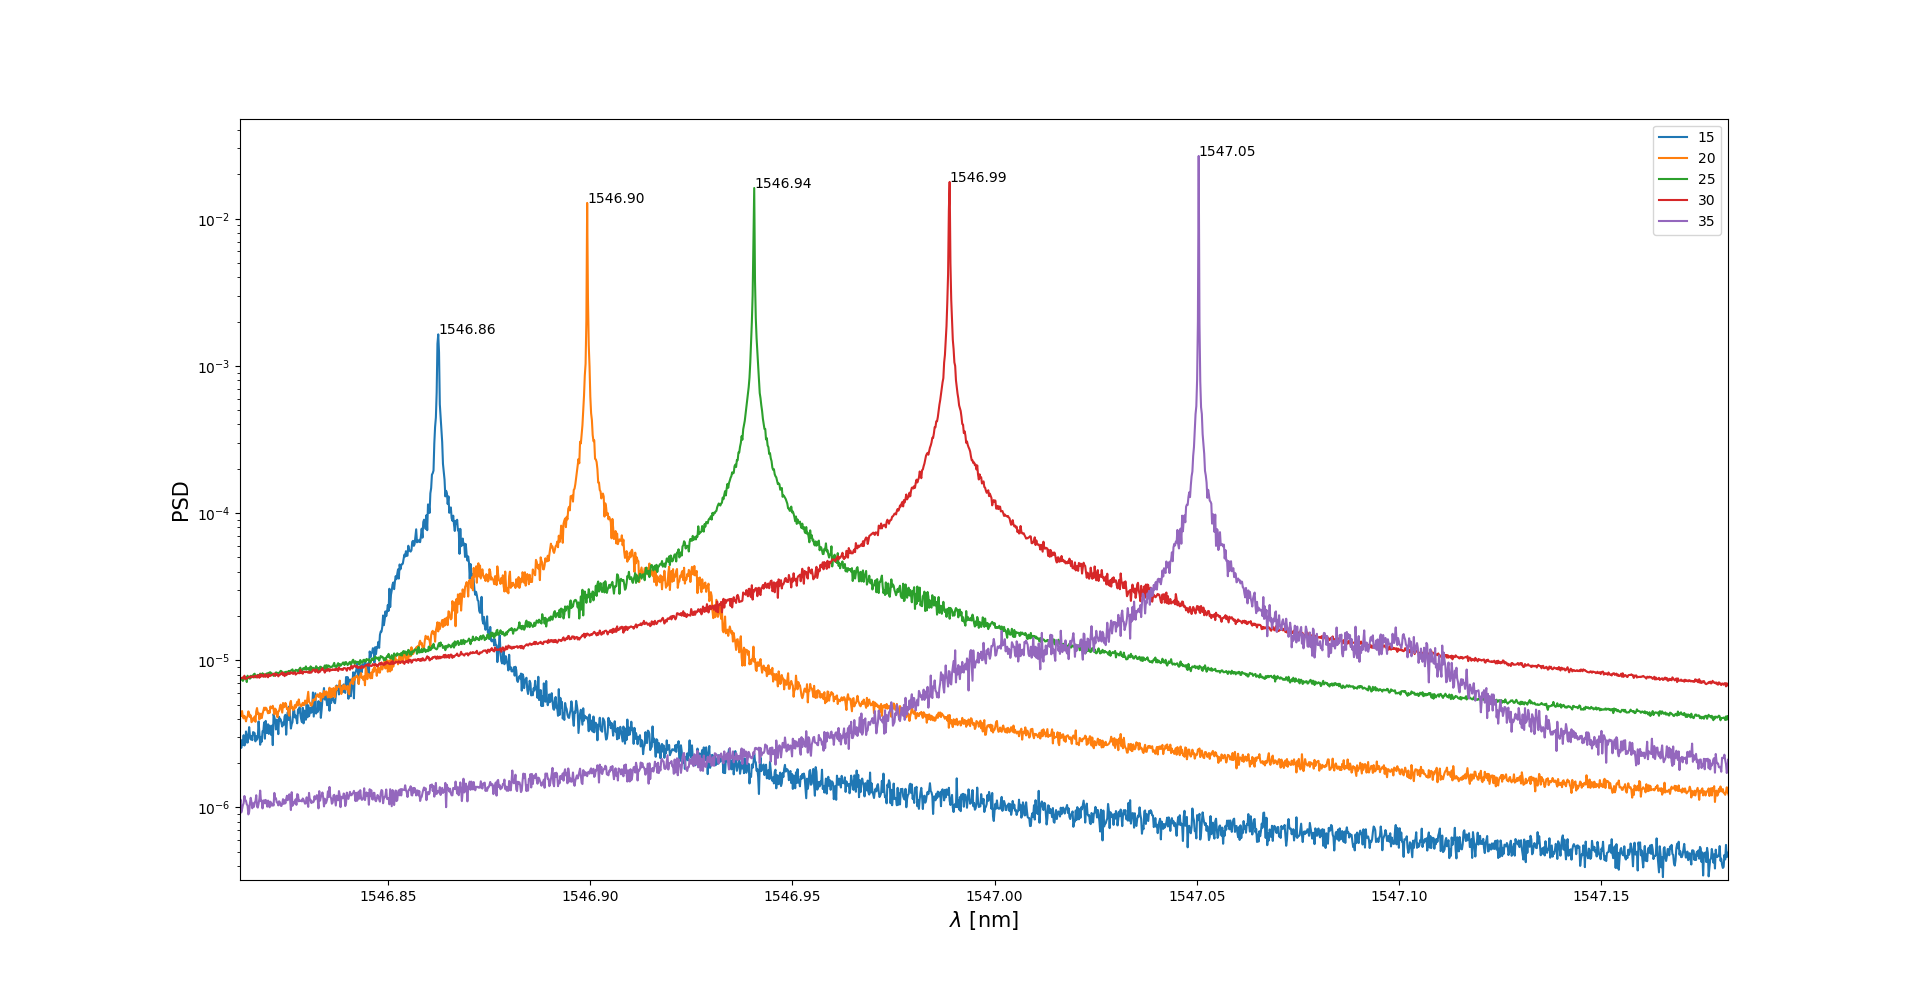
\includegraphics[width=1.0\linewidth]{Espectros.png}
			\caption{\label{Img:widgets}Espectros en continua de la simulacion}
		\end{figure}

		\begin{table}[H]
			\centering
			\begin{tabular}{c c}
				\hline
				$I_{Bias}$ & $\lambda$ \\\hline 
				15 & 1546.86 \\
				20 & 1546.90 \\
				25 & 1546.94 \\
				30 & 1546.99 \\
				35 & 1547.05 \\\hline
			\end{tabular}
			\caption{\label{tab:label}Lambdas de la simulacion}
		\end{table}

		\begin{figure}[H]
			\centering
			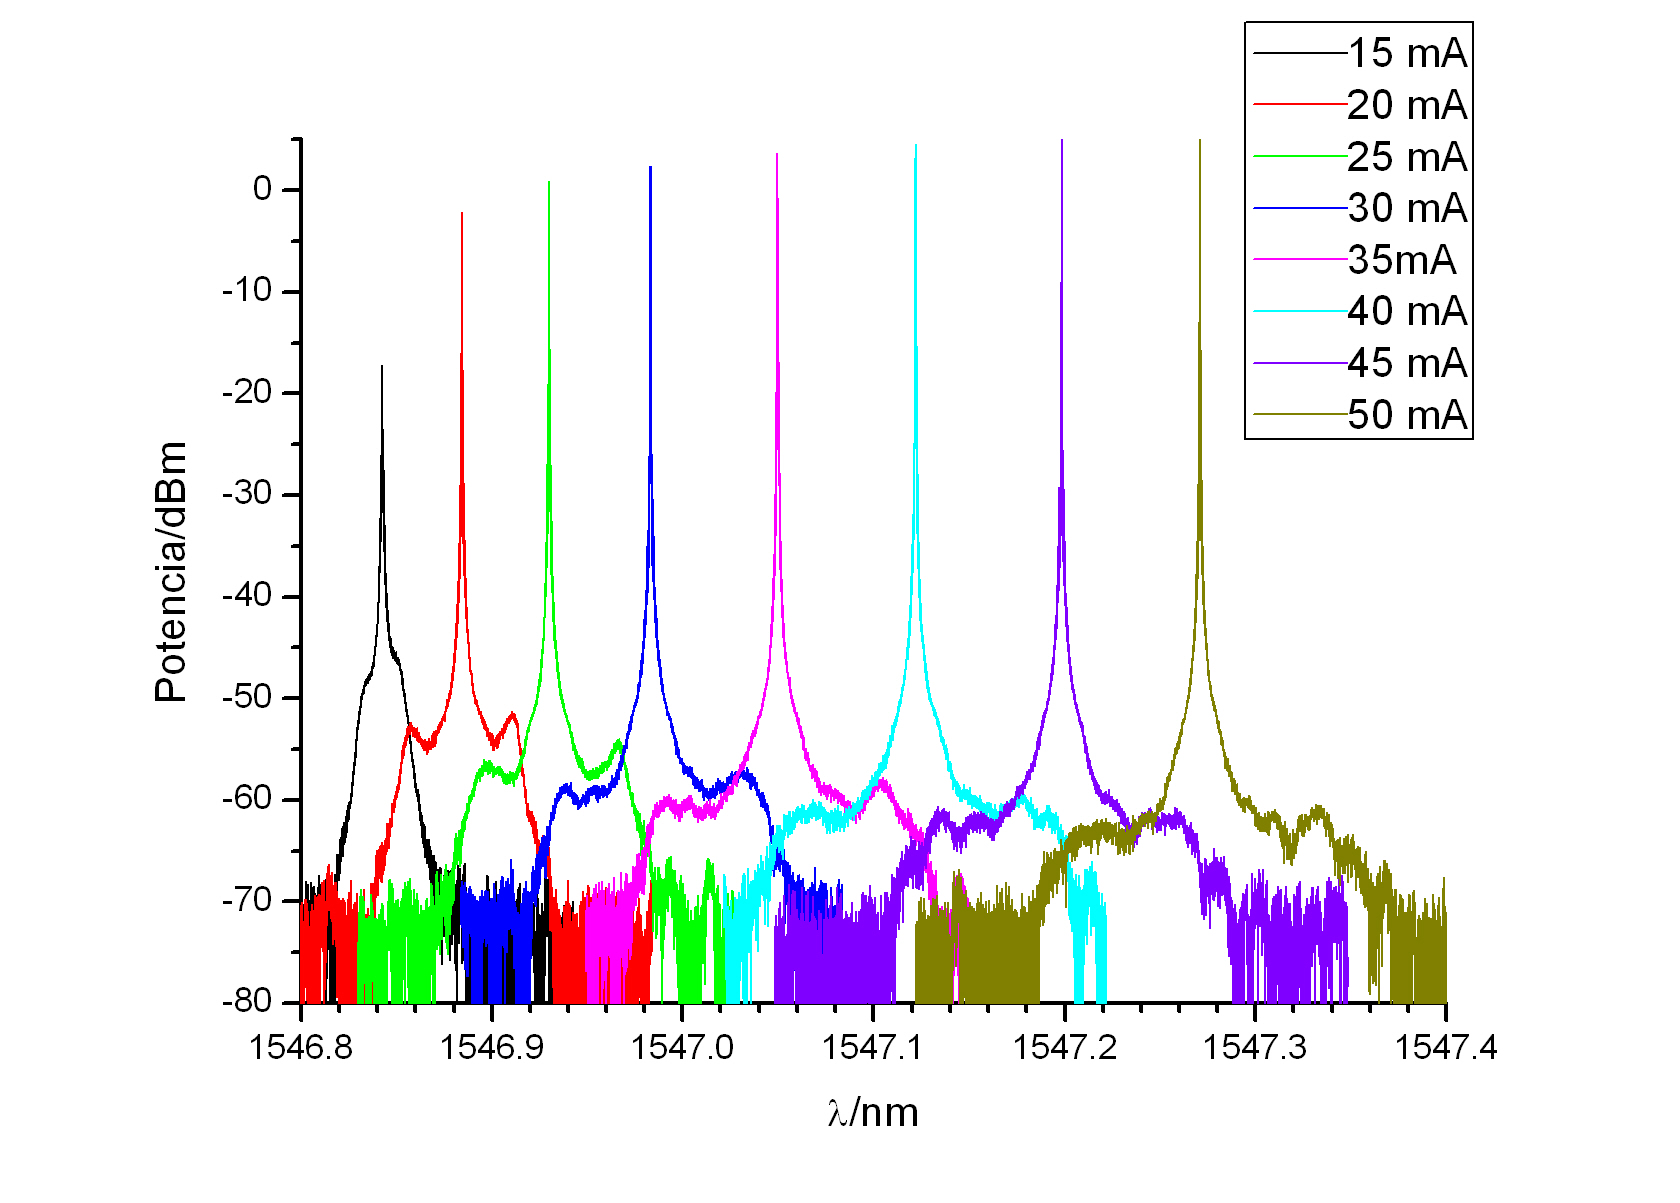
\includegraphics[width=1.0\linewidth]{../Chaves/OFC-GS/EspectrosT25.jpg}
			\caption{\label{fig:EspectrosT25}Espectros en continua de Chaves}	
		\end{figure}
	

		\begin{figure}[H]
			\centering
			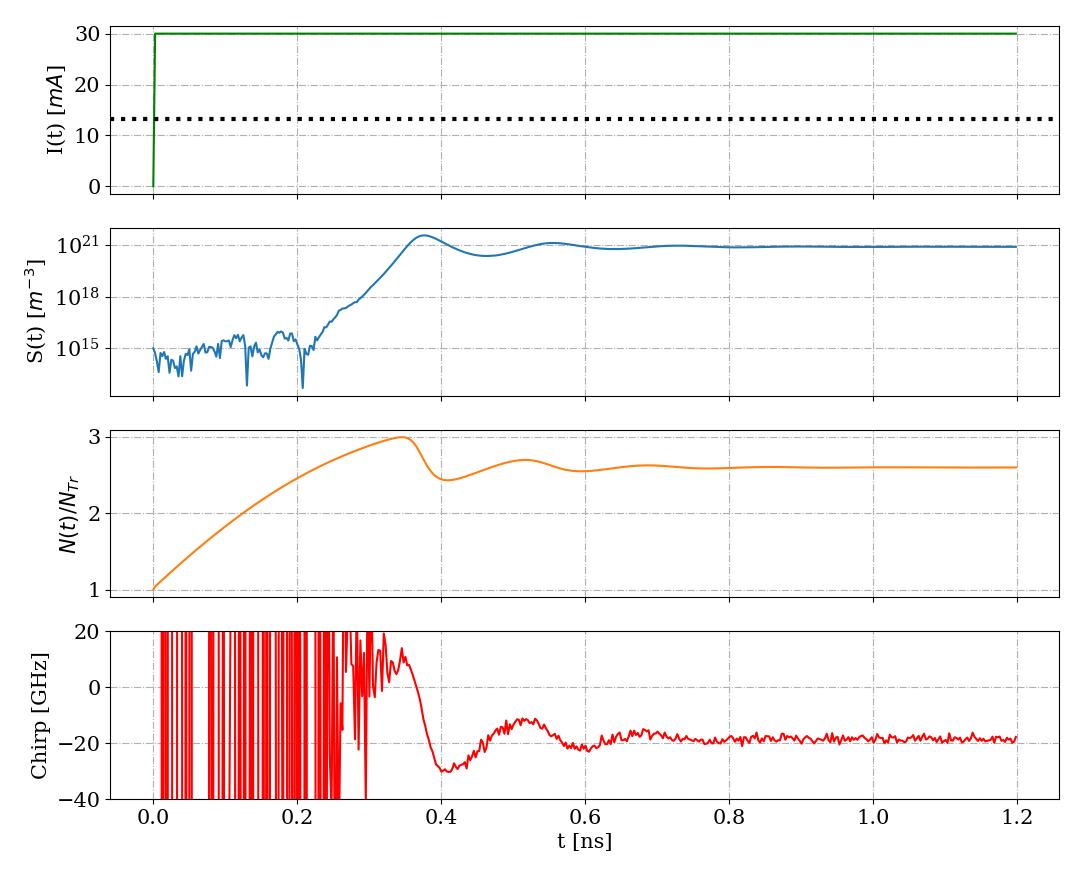
\includegraphics[width=1.0\linewidth]{transitorio.png}
			\caption{\label{fig:transitorio}Transitorio}	
		\end{figure}

		\begin{figure}[H]
			\centering
			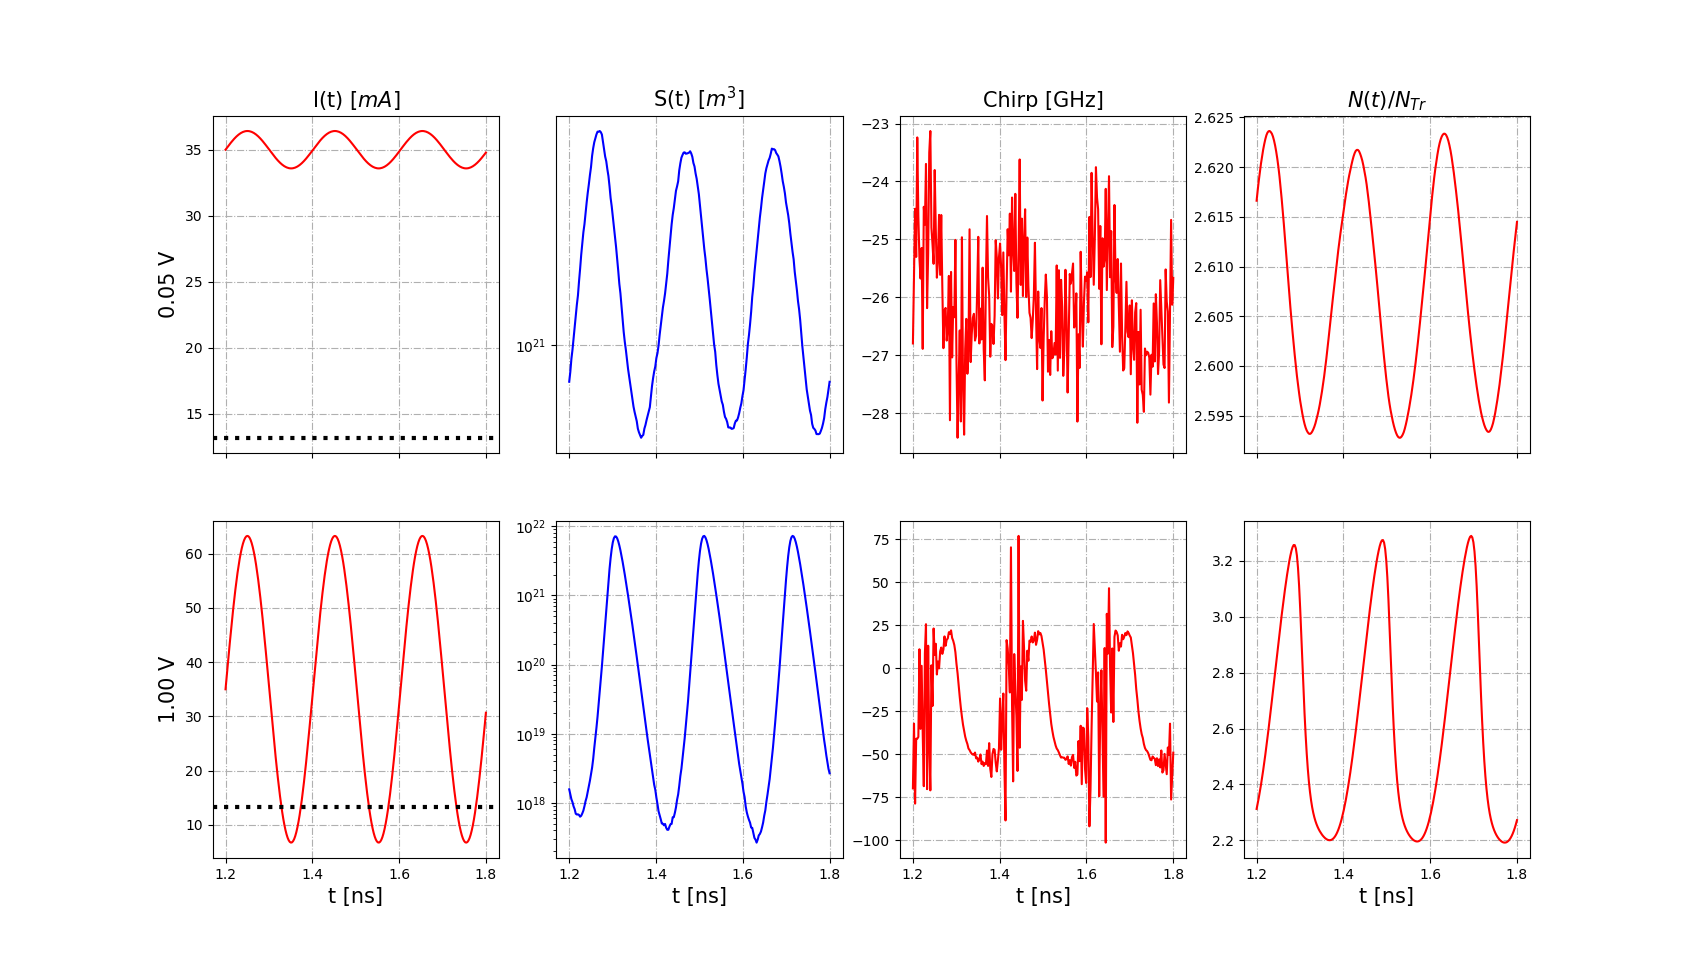
\includegraphics[width=1.0\linewidth]{rateEquations.png}
			\caption{\label{fig:rateEquations}RateEquations}	
		\end{figure}

		\begin{figure}[H]
			\centering
			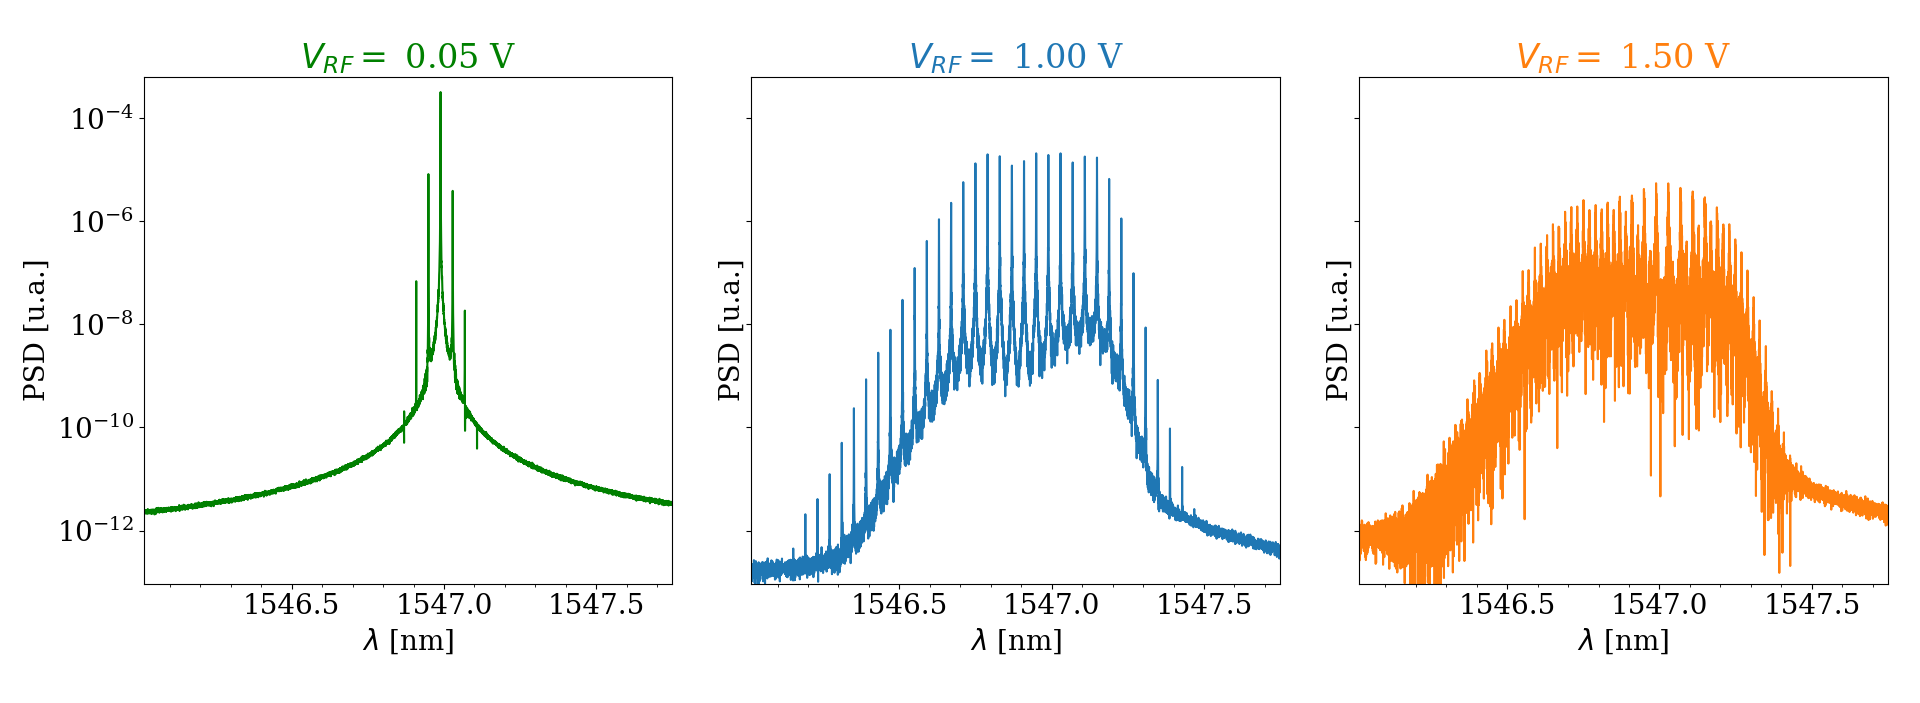
\includegraphics[width=1.0\linewidth]{PSD.png}
			\caption{\label{fig:PSD}PSD}	
		\end{figure}

		\begin{figure}[H]
			\centering
			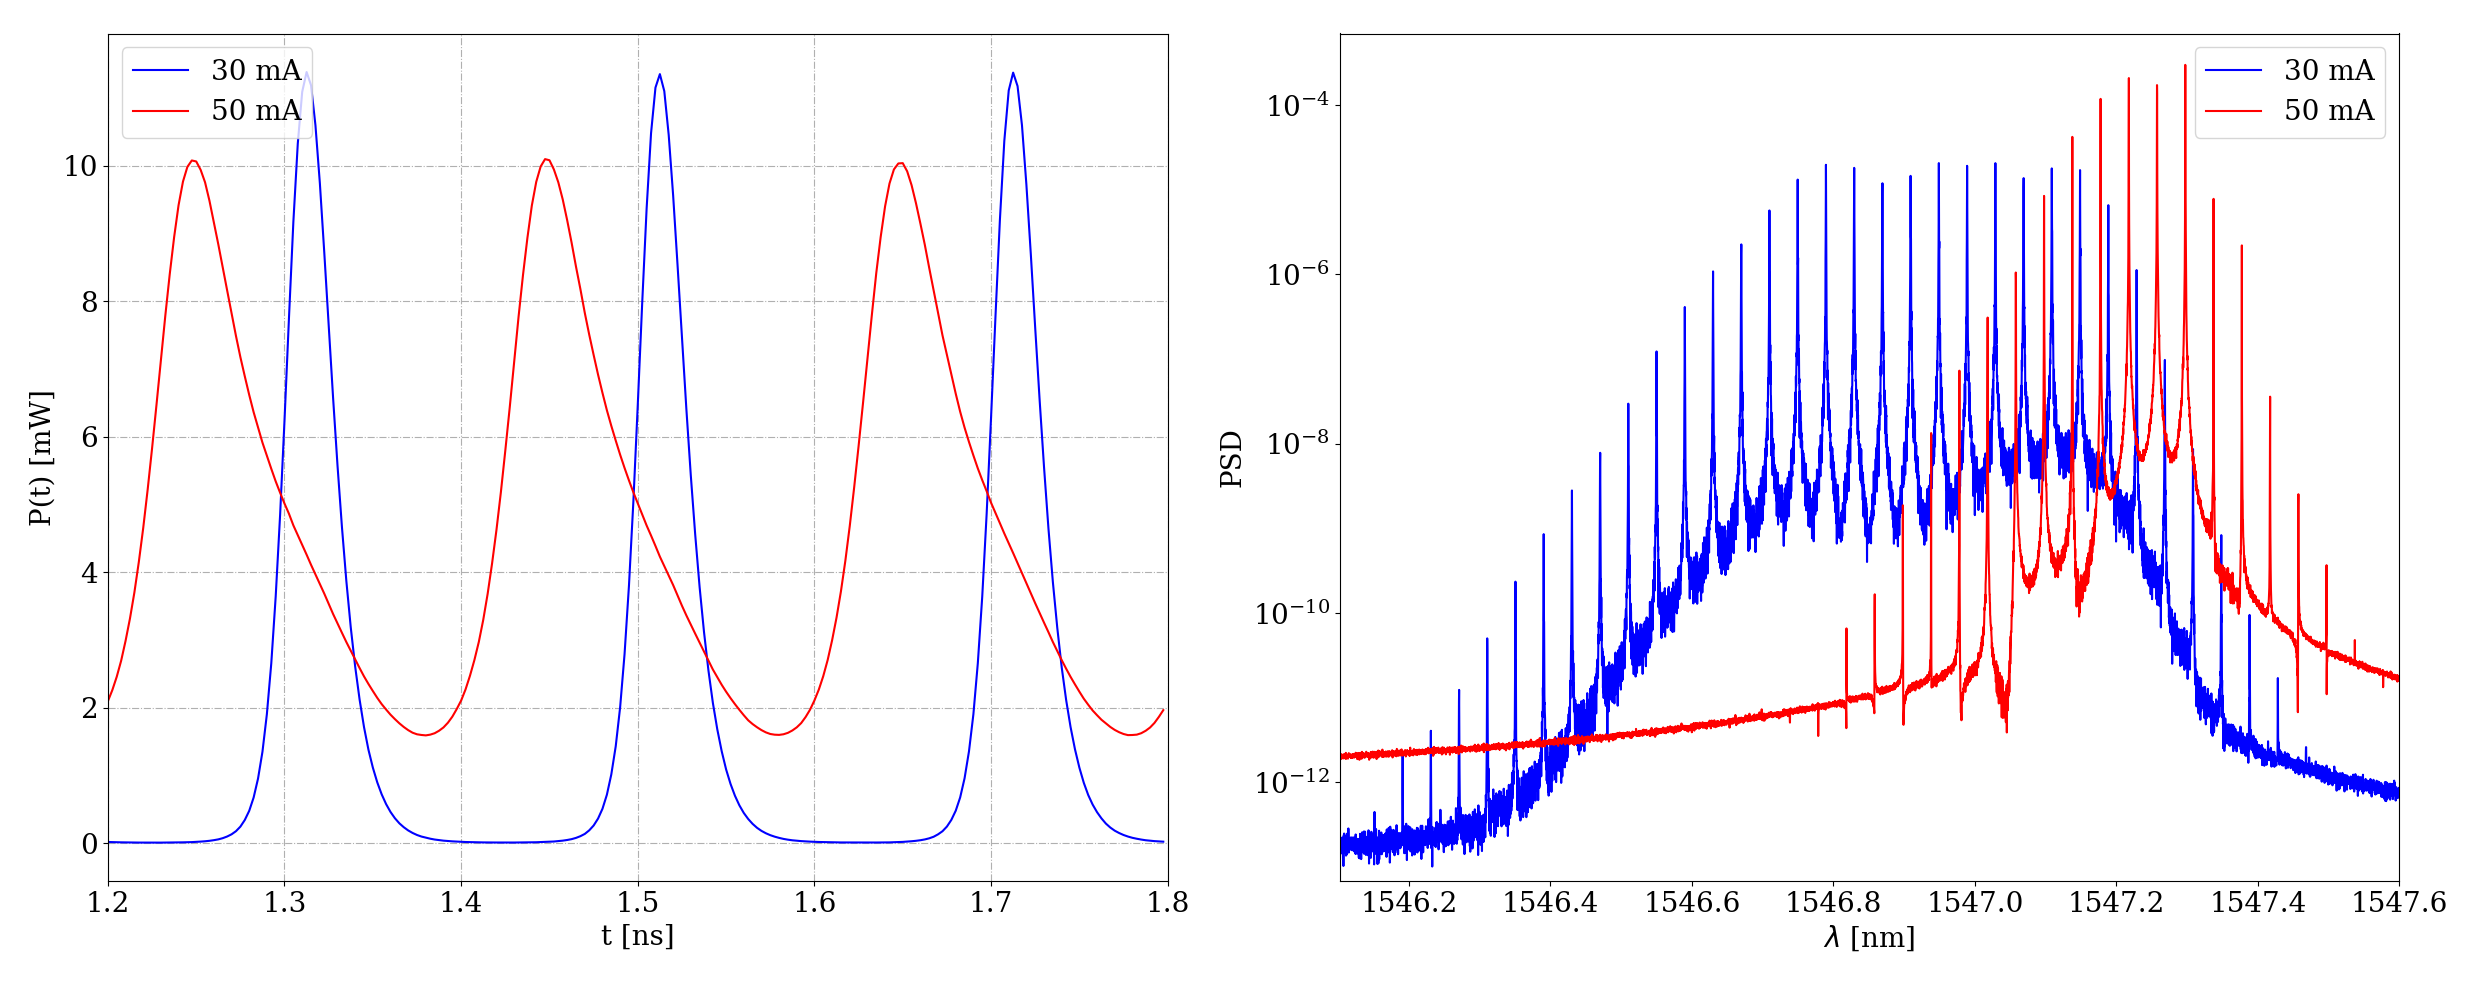
\includegraphics[width=1.0\linewidth]{current.png}
			\caption{\label{fig:current}Current}	
		\end{figure}

		\begin{figure}[H]
			\centering
			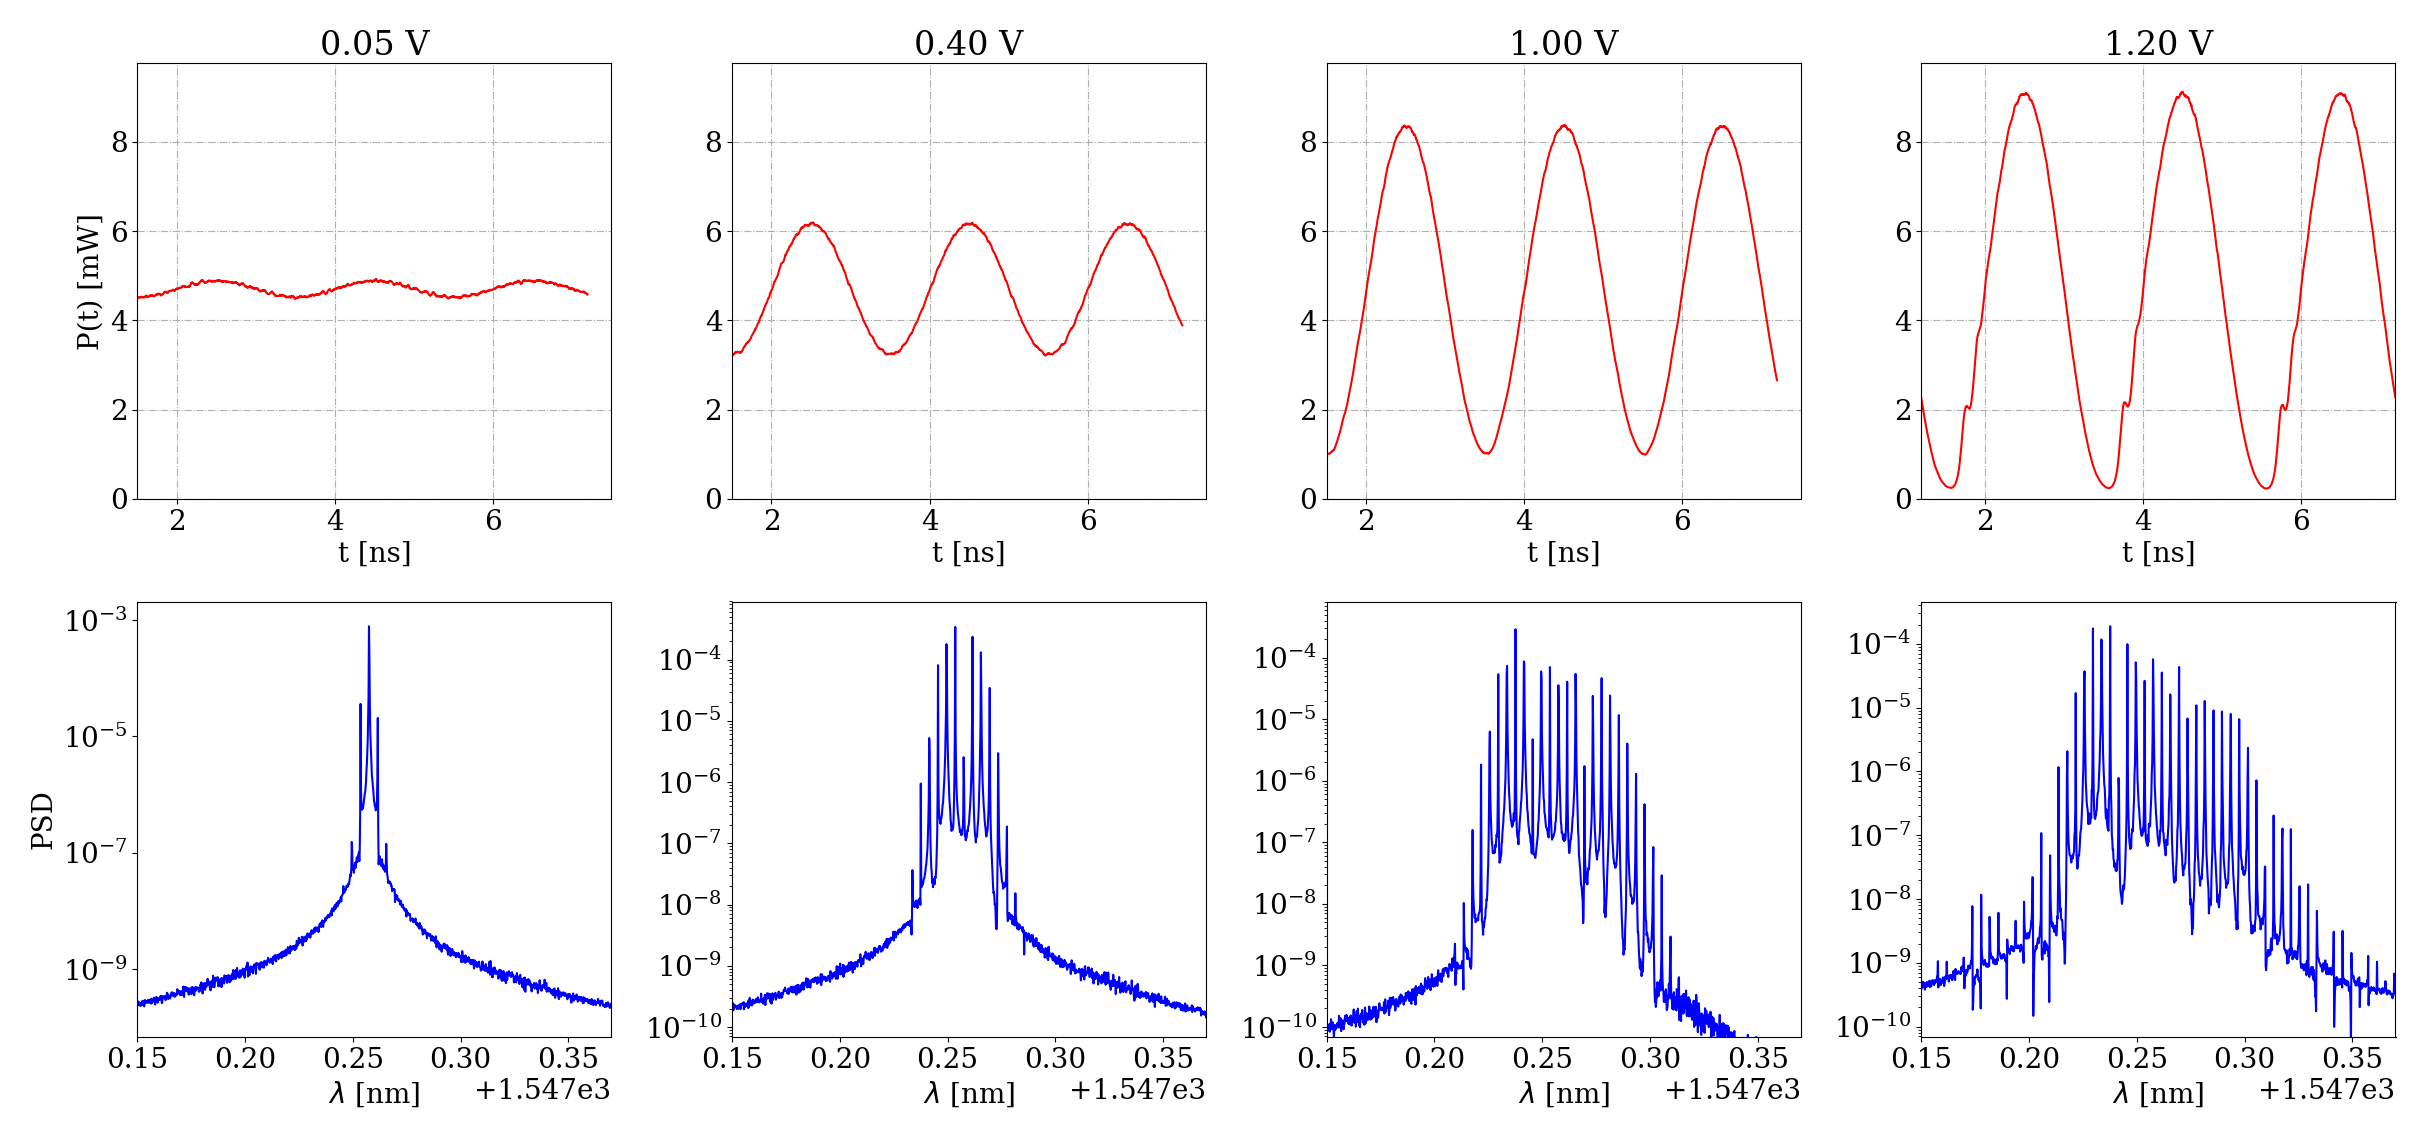
\includegraphics[width=1.0\linewidth]{500.png}
			\caption{\label{fig:500}500}	
		\end{figure}

		\begin{figure}[H]
			\centering
			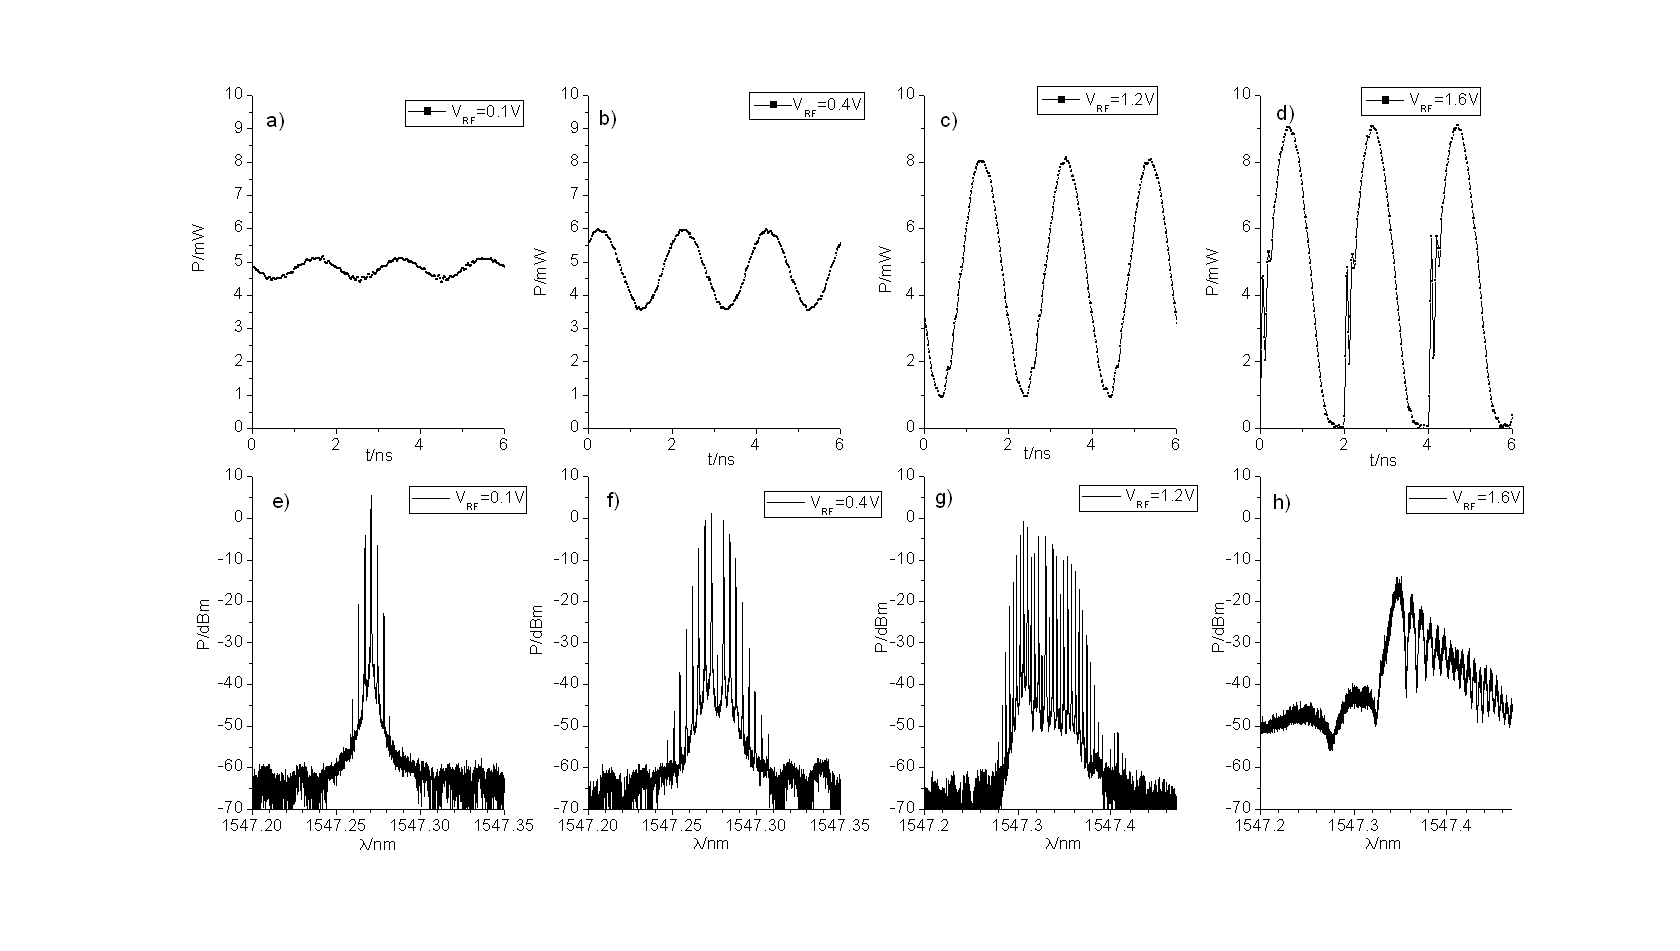
\includegraphics[width=1.0\linewidth]{../Chaves/OFC-GS/500mhz.png}
			\caption{\label{fig:500mhz}500mhz}	
		\end{figure}


	

			\addtocontents{toc}{\vspace{0.1cm}}
			\chapter{Inyeccion de Luz}

				\graphicspath{{../Graphics/Cpt2-InjectCW/}}


			\begin{figure}[H]
				\centering
				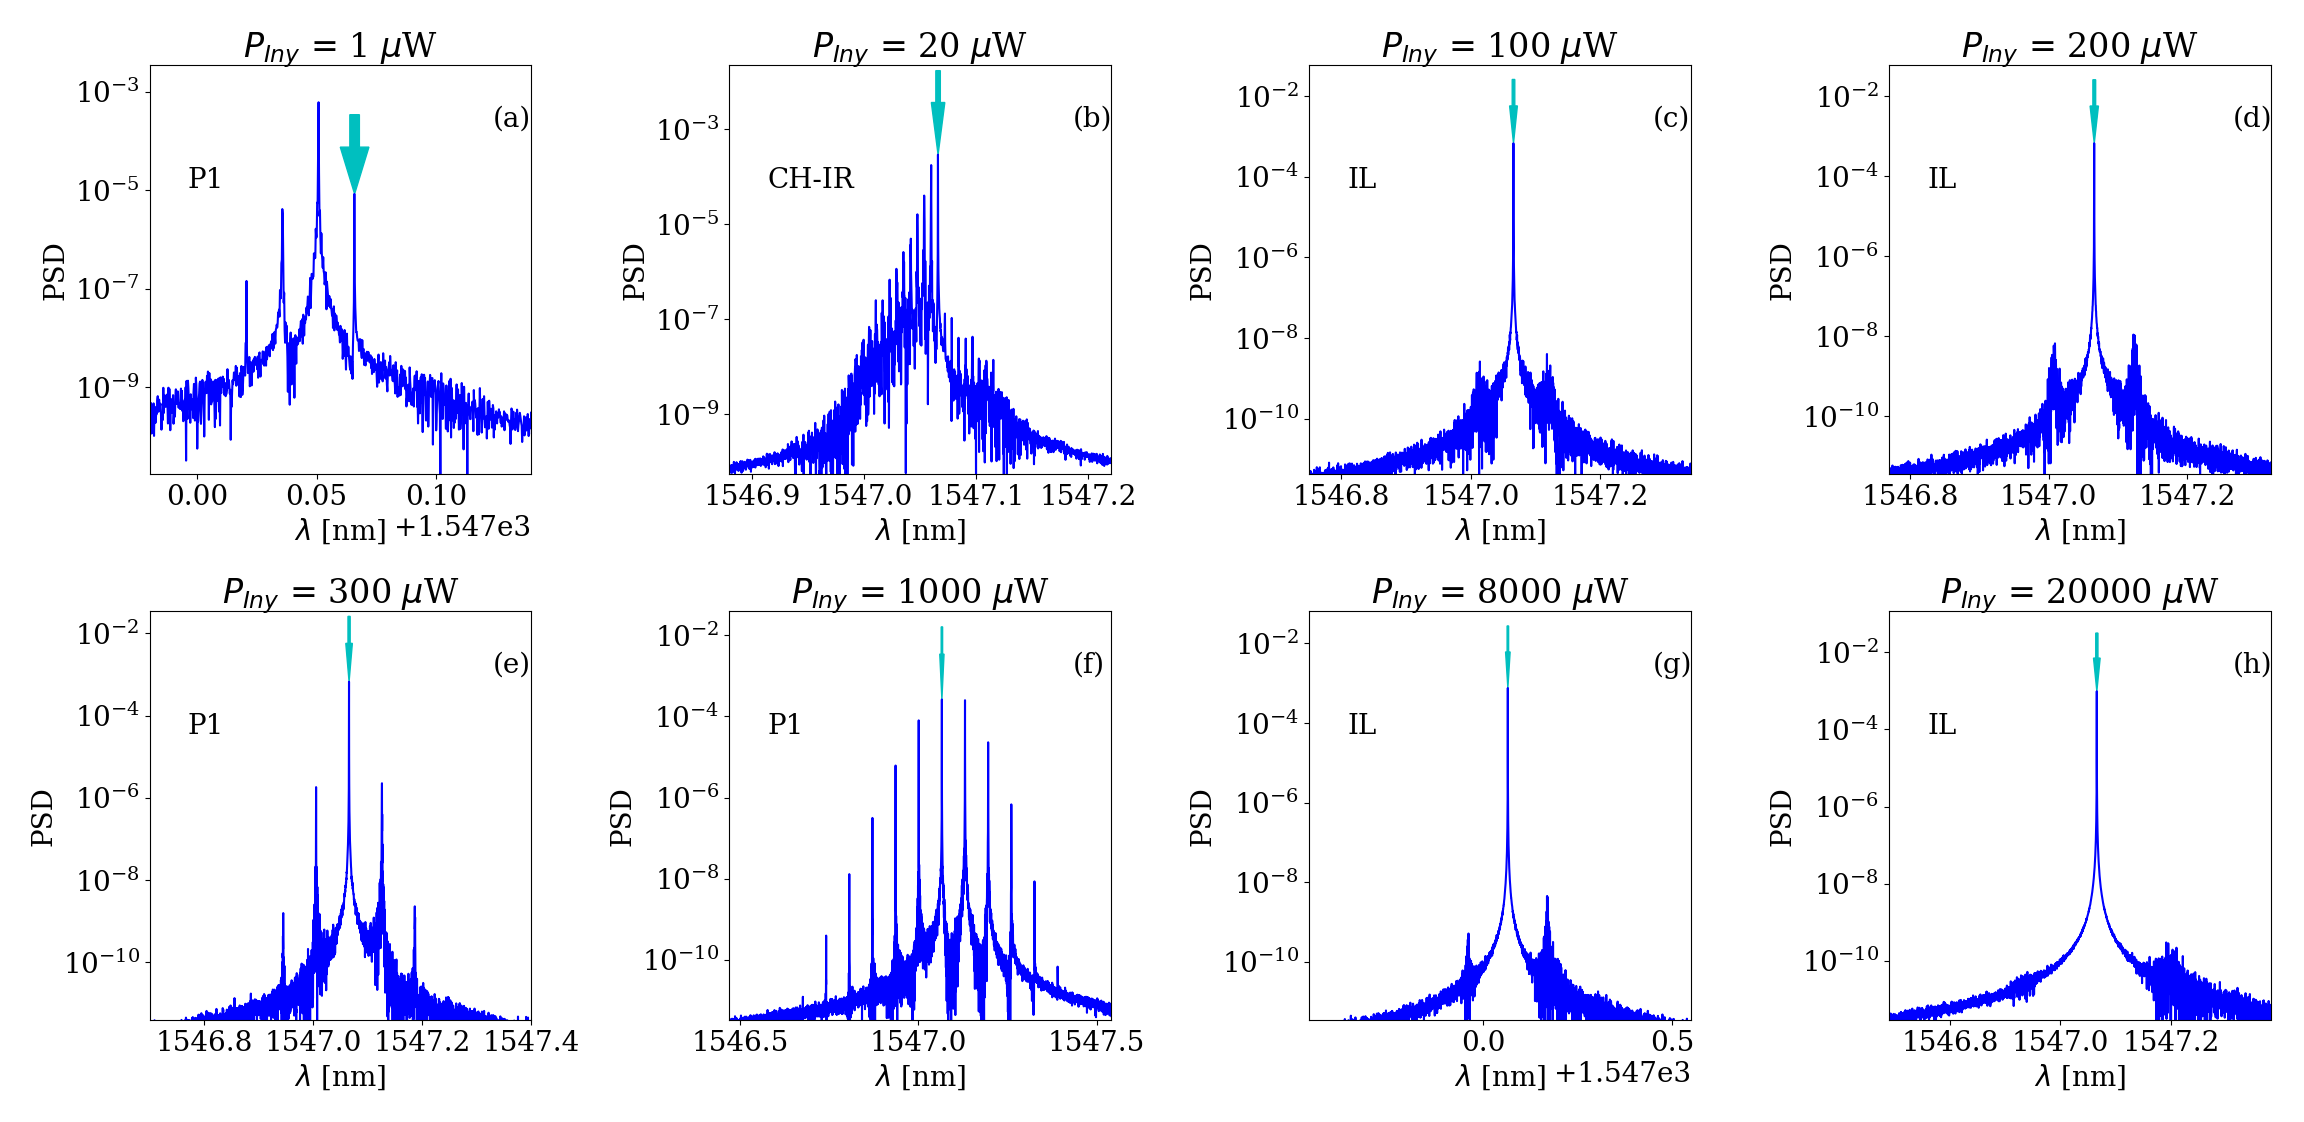
\includegraphics[width=1.0\linewidth]{zoneMap.png}
				\caption{\label{Img:widgets}el pie de pagina que le quieras 	poner a la imagen}
			\end{figure}

			\begin{figure}[H]
				\centering
				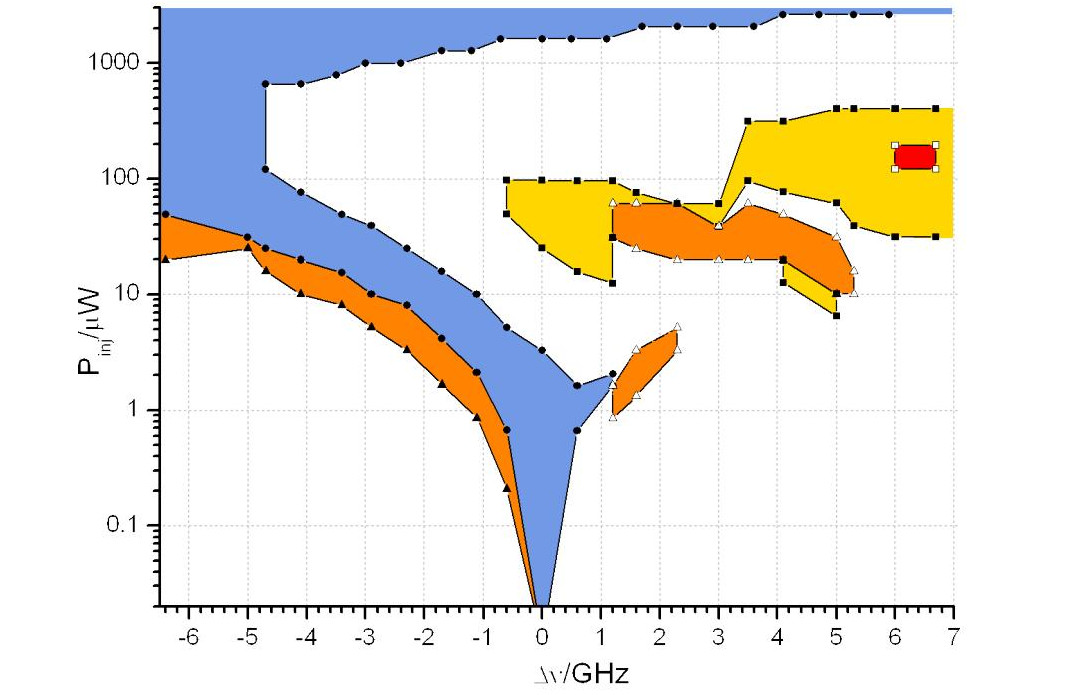
\includegraphics[width=1.0\linewidth]{mapa.jpg}
				\caption{\label{fig:map}Map}	
			\end{figure}

			\begin{figure}[H]
				\centering
				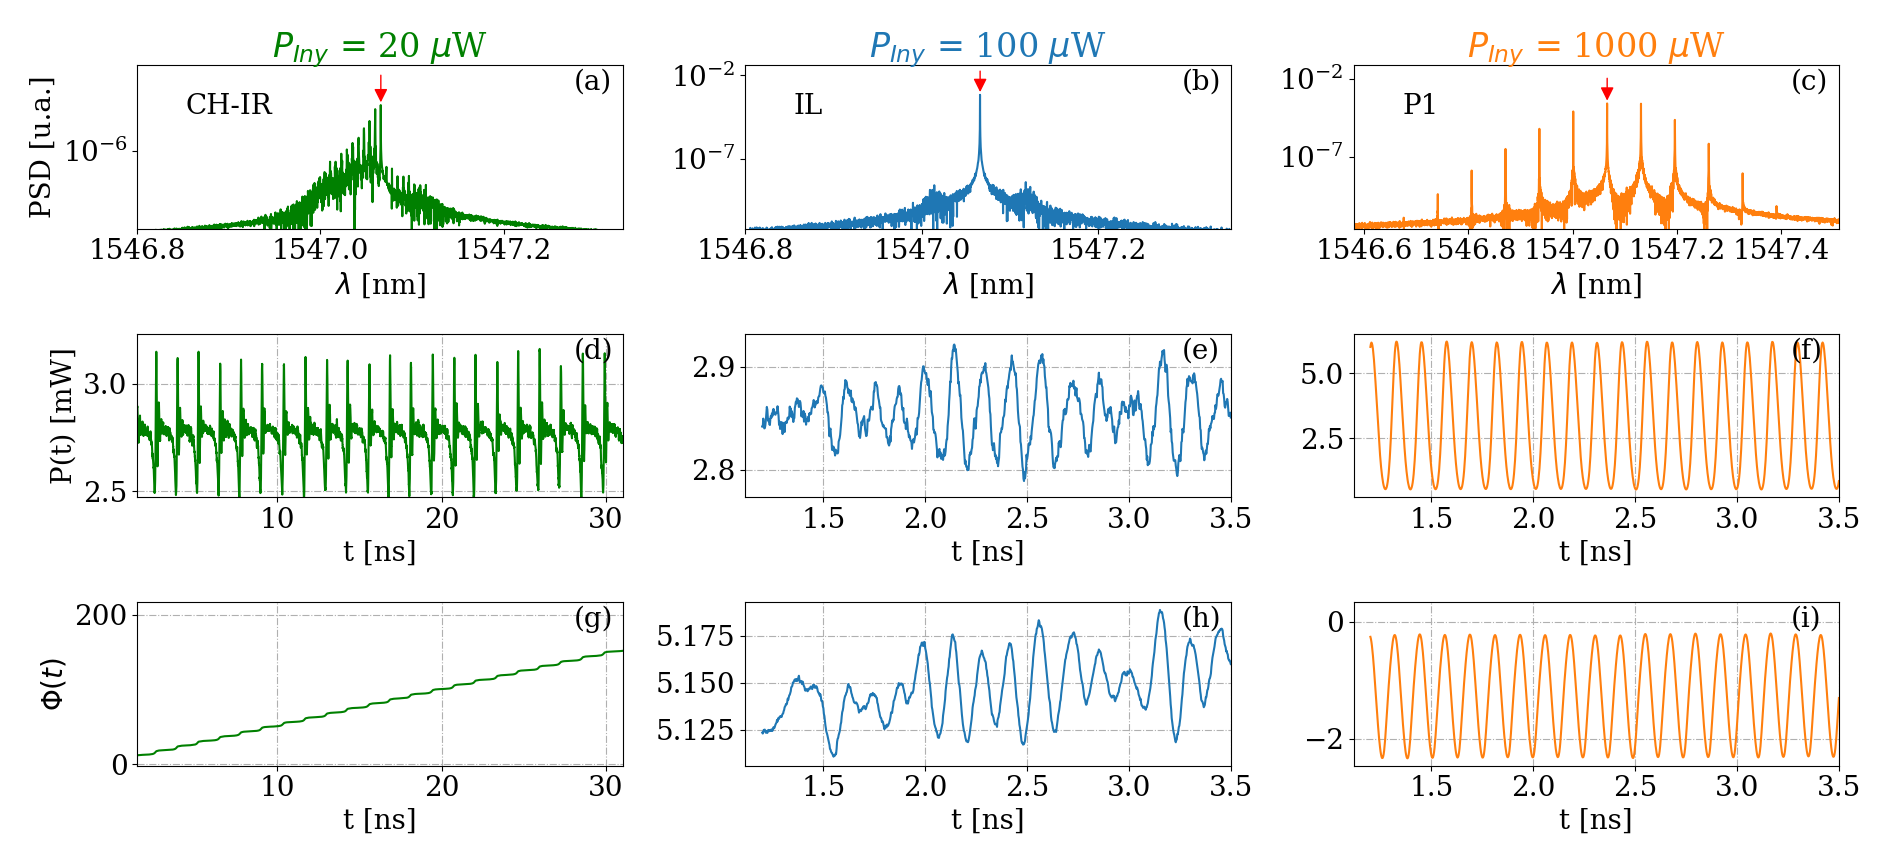
\includegraphics[width=1.0\linewidth]{zoneRtEq.png}
				\caption{\label{fig:zoneRtEq}ZoneRtEq}	
			\end{figure}

			\begin{figure}[H]
				\centering
				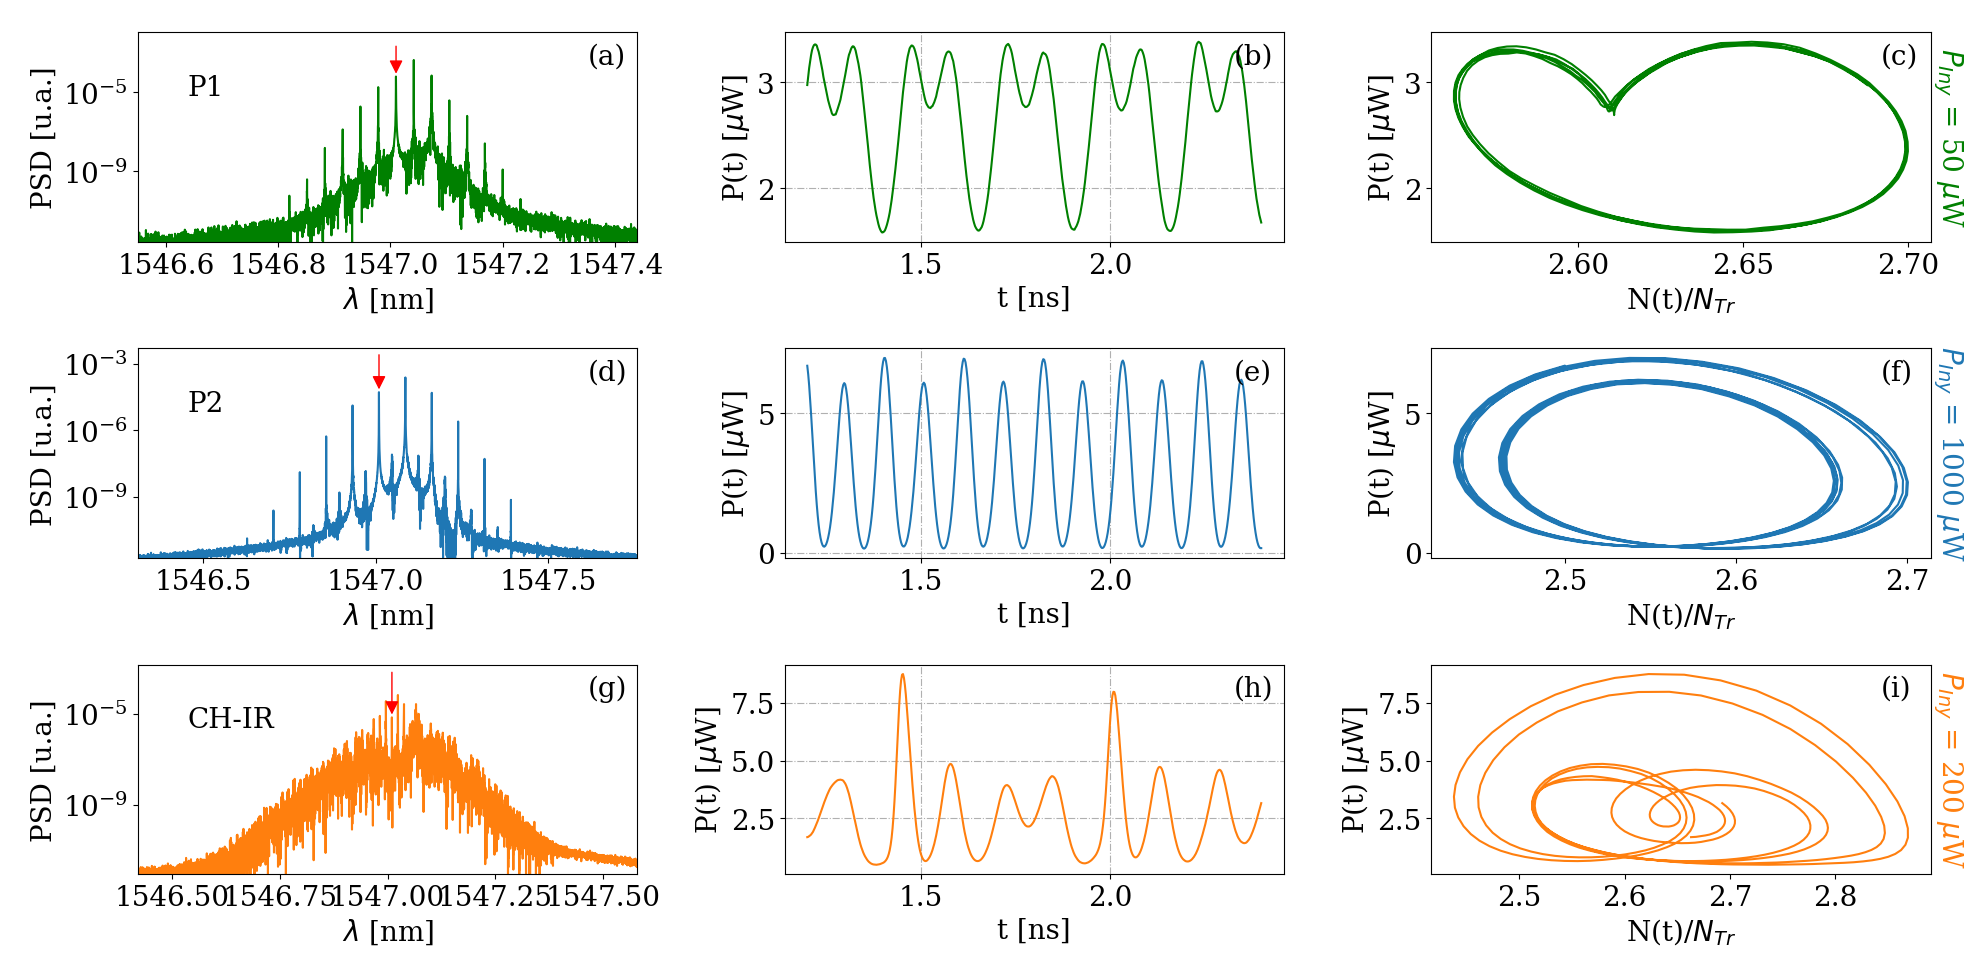
\includegraphics[width=1.0\linewidth]{P2zone.png}
				\caption{\label{fig:P2zone}P2zone}	
			\end{figure}


				
			\addtocontents{toc}{\vspace{0.1cm}}
			\chapter{Inyeccion de luz en OFC}

				\graphicspath{{../Graphics/Cpt3-CombInject/}}

En este cap\'itulo se han combinado los m\'etodos de generaci\'on de OFC estudiados en los cap\'itulos anteriores, abordando el estudio de los r\'egimenes din\'amicos que existen en la generaci\'on de OFC mediante \gs\ e inyecci\'on de luz. Se ha trabajado con el l\'aser ML con $\ibias = 35$ mA, $V_{RF} = 1.$ V y alta frecuencia $f_R = 5$ GHz. Para las condiciones de inyecci\'on de SL se ha tomado un \'unico valor de $\delta\nu = -2$ GHz, variando la potencia de inyecci\'on $P_{Iny}$.

En la Figura \ref{Img:MapGS-IO} se muestran los espectros \'opticos de las diferentes regiones din\'amicas obtenidas para distintas $P_{Iny}$ a $\delta\nu = -2$ GHz. 


			\begin{figure}[H]
				\centering
				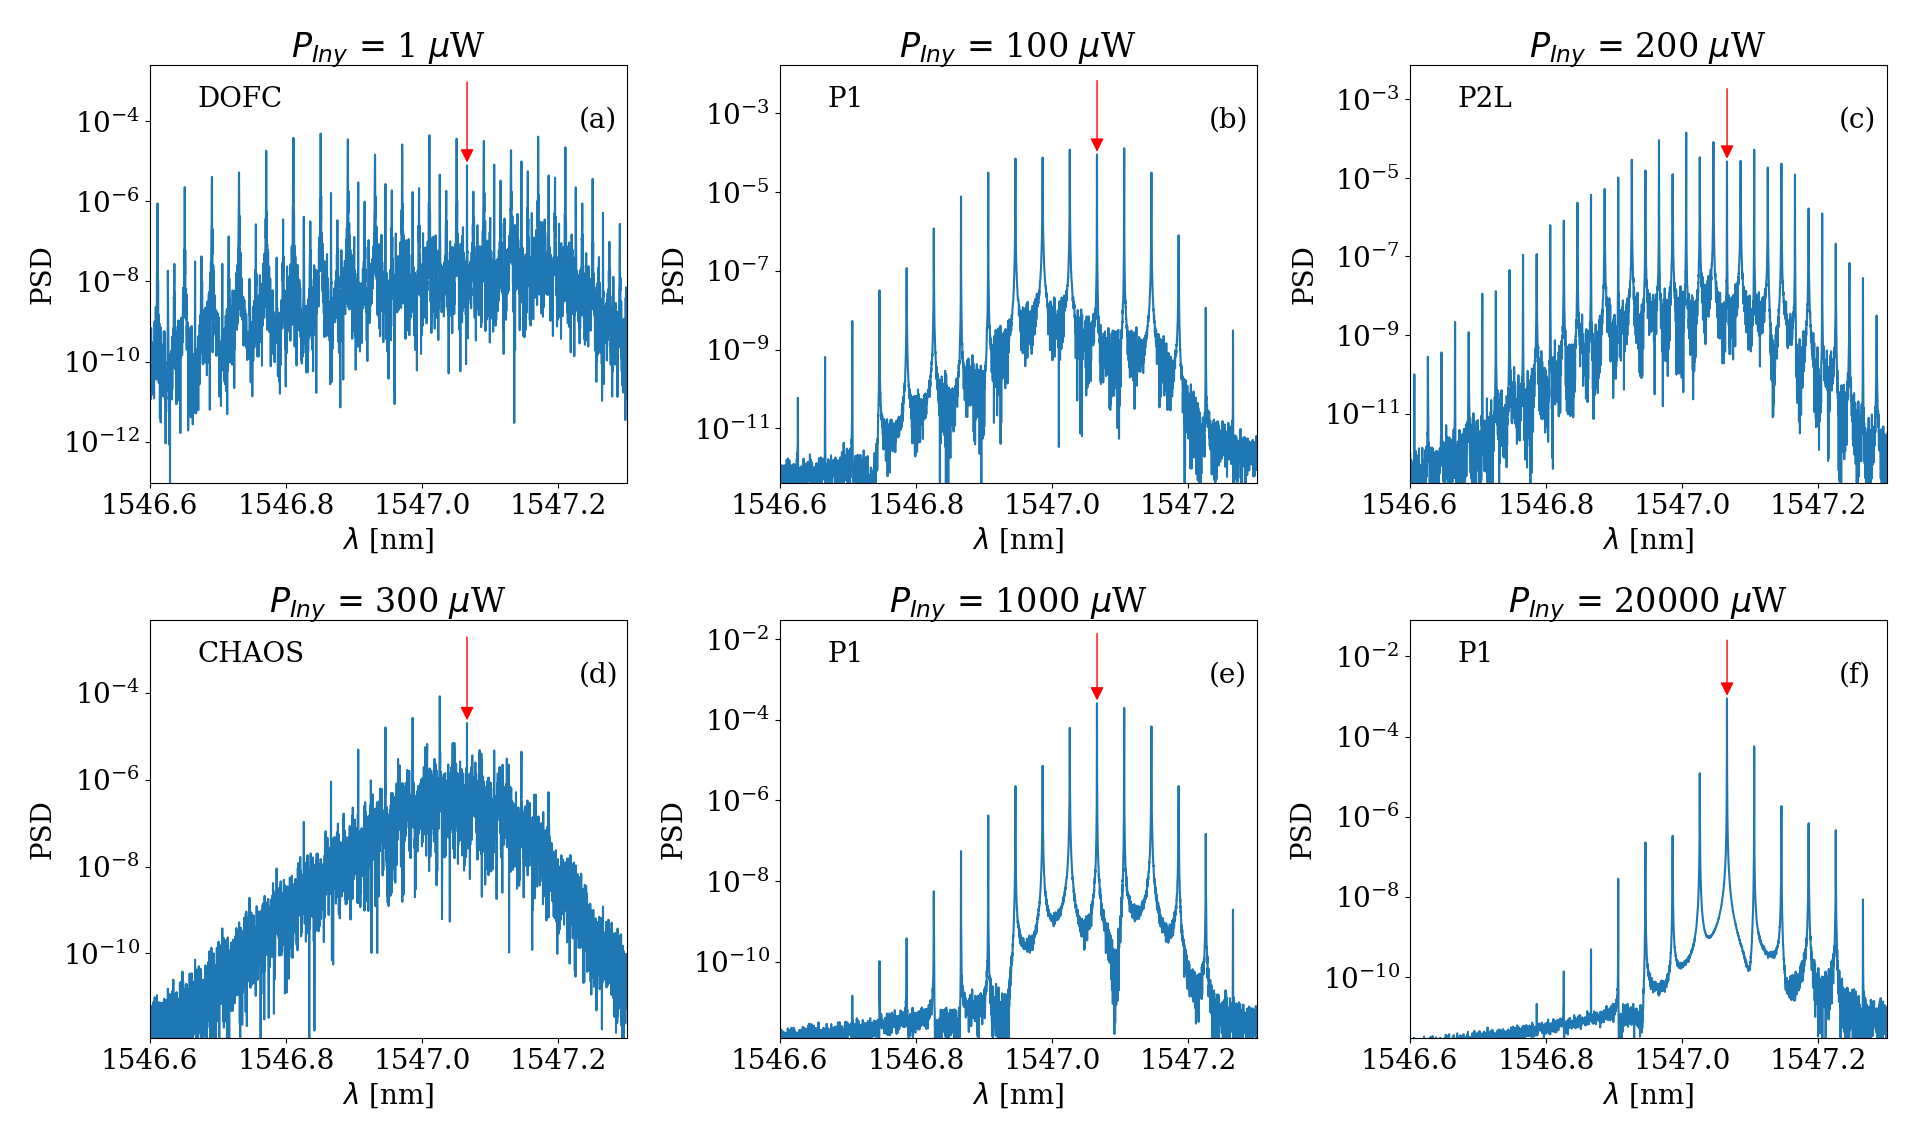
\includegraphics[width=1.0\linewidth]{psdMap.png}
				\caption{\label{Img:MapGS-IO}Espectros \'opticos obtenidos mediante \gs\ e inyección \'optica de las diferentes regiones dinámicas obtenidas para diferentes $P_{Iny}$ a $\delta\nu = -2$ GHz. Se indica la frecuencia de inyección $\nu_{SL}$ con una flecha y $P_{Iny}$ para cada espectro \'optico.}
			\end{figure}

		Para $P_{Iny} = 1\;\mu$W se obtiene un espectro \'optico con doble peine \'optico de frecuencias, DOFC, observando dos picos de emisión a cada lado del OFC principal (Figura \ref{Img:MapGS-IO} (a)). El DOFC se desruye al aumentar la potencia de inyección, obteniendo un OFC simple en la regi\'on P1 para $P_{Iny} = 100\;\mu$W (Figura \ref{Img:MapGS-IO} (b)). Al aumentar $P_{Iny} = 200 \;\mu$W se produce un doblamiento de periodo P2, obteniendo un OFC cuyas frecuencias de separaci\'on entre pico es la mitad que para la regi\'on P1 (Figura \ref{Img:MapGS-IO} (c)). La región de caos, CHAOS, se obtiene para $P_{Iny} = 300\;\mu$W, para la que el OFC se destruye (Figura \ref{Img:MapGS-IO} (d)). Con altas potencias de inyecci\'on $P_{Iny} = 1000\;\mu$W y $ 20000\;\mu$W se alcanza nuevamente la regi\'on P1 con un pico m\'aximo para la frecuencia de inyecci\'on $\nu_{SL}$. Dentro de esta regi\'on, al aumentar $P_{Iny}$ tanto el ruido debido a la emisi\'on espont\'anea como los picos de emisi\'on que se encuentran a los lados del pico en $\nu_{SL}$ disminuyen, mientras que el pico co nla frecuencia de inyecci\'on aumenta. Esta tendencia puede indicar la existencia de una nueva regi\'on con IL para $P_{Iny}$ superiores a los valores con los que se ha trabajado.

		Se han estudiado y comparado algunos casos concretos de las regiones mostradas en la Figura \ref{Img:MapGS-IO}, analizando el comportamiento de las variables internas con el objetivo de entender mejor los fen\'omenos que se producen en cada caso, de cara a realizar una correcta distinci\'on de las diferentes regiones din\'amicas.

		En la Figura \ref{fig:p1-p2} se muestran los espectros \'opticos, $P(t)$ y el atractor en el espacio de los estados de las ecuaciones de balance, despreciando los efectos de la fase \'optica; para $\delta\nu = -2$GHz y $P_{Iny} = 100\;\mu$W y $200\;\mu$W.

			\begin{figure}[H]
				\centering
				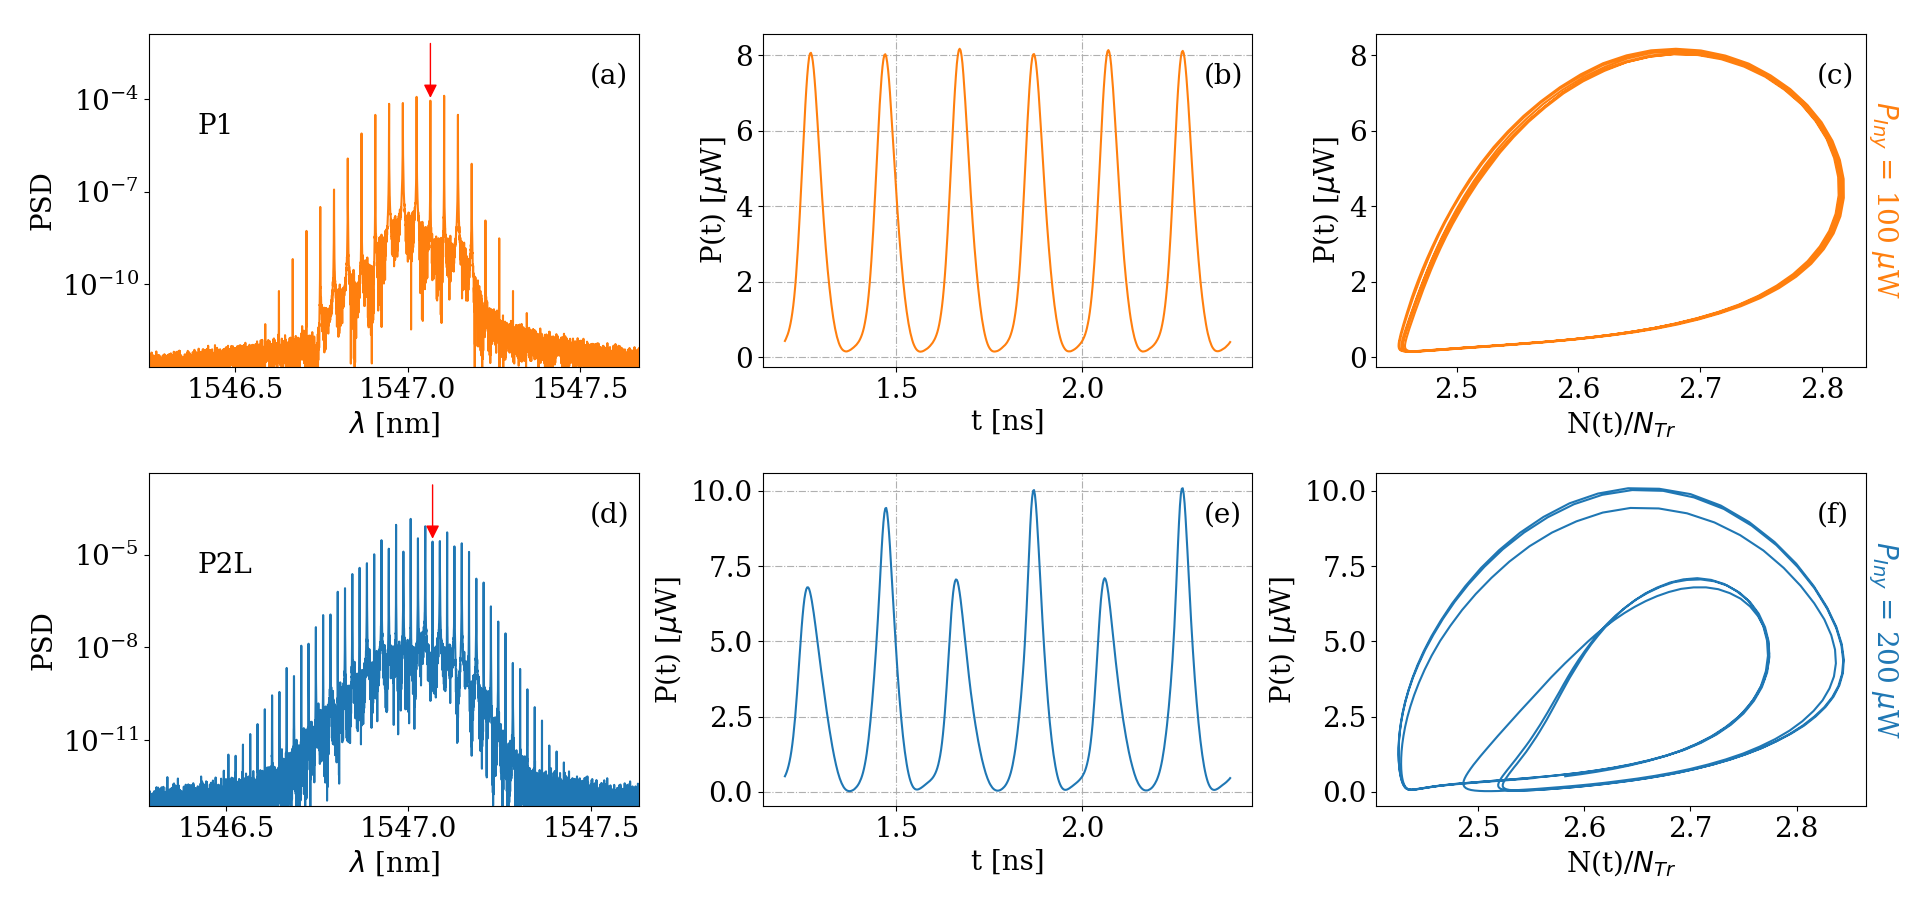
\includegraphics[width=1.0\linewidth]{p1-p2.png}
				\caption{\label{fig:p1-p2}Espectros \'opticos, $P(t)$ y atractor en el espacio de los estados de las ecuaciones de balance, despreciando los efectos de la fase \'optica; para $\delta\nu = -2$GHz y $P_{Iny} = 100\;\mu$W (P1, naranja) y $200\;\mu$W (P2, azul).}	
			\end{figure}

		Los resultados de la Figura \ref{fig:p1-p2} permiten comparar m\'s a fondo las regiones P1 y P2, obteniendo para ambos casos dos OFC con similares perfiles pero cuya separaci\'on entre l\'ineas es la mitad para el caso de P2. Esto se puede observar en la Figura \ref{fig:p1-p2} (e) en la que la diferencia de amplitudes entre picos continuos produce que el periodo de las oscilaciones de $P(t)$ no sea el tiempo entre picos continuas, sino el tiempo entre picos con la misma amplitud, que es el doble. Tambi\'en se puede observar en la Figura \ref{fig:p1-p2} (f) en la que se obtiene una doble oscilación con un diagrama similar al de la Figura \ref{fig:P2zon} (f) para la regi\'on P2 del c\'apitulo anterior.

		En la Figura \ref{fig:chaos} se muestran los espectros \'opticos, $P(t)$ y el atractor en el espacio de los estados de las ecuaciones de balance, despreciando los efectos de la fase \'optica; para $\delta\nu = -2$GHz y $P_{Iny} = 1\;\mu$W y $300\;\mu$W.

			\begin{figure}[H]
				\centering
				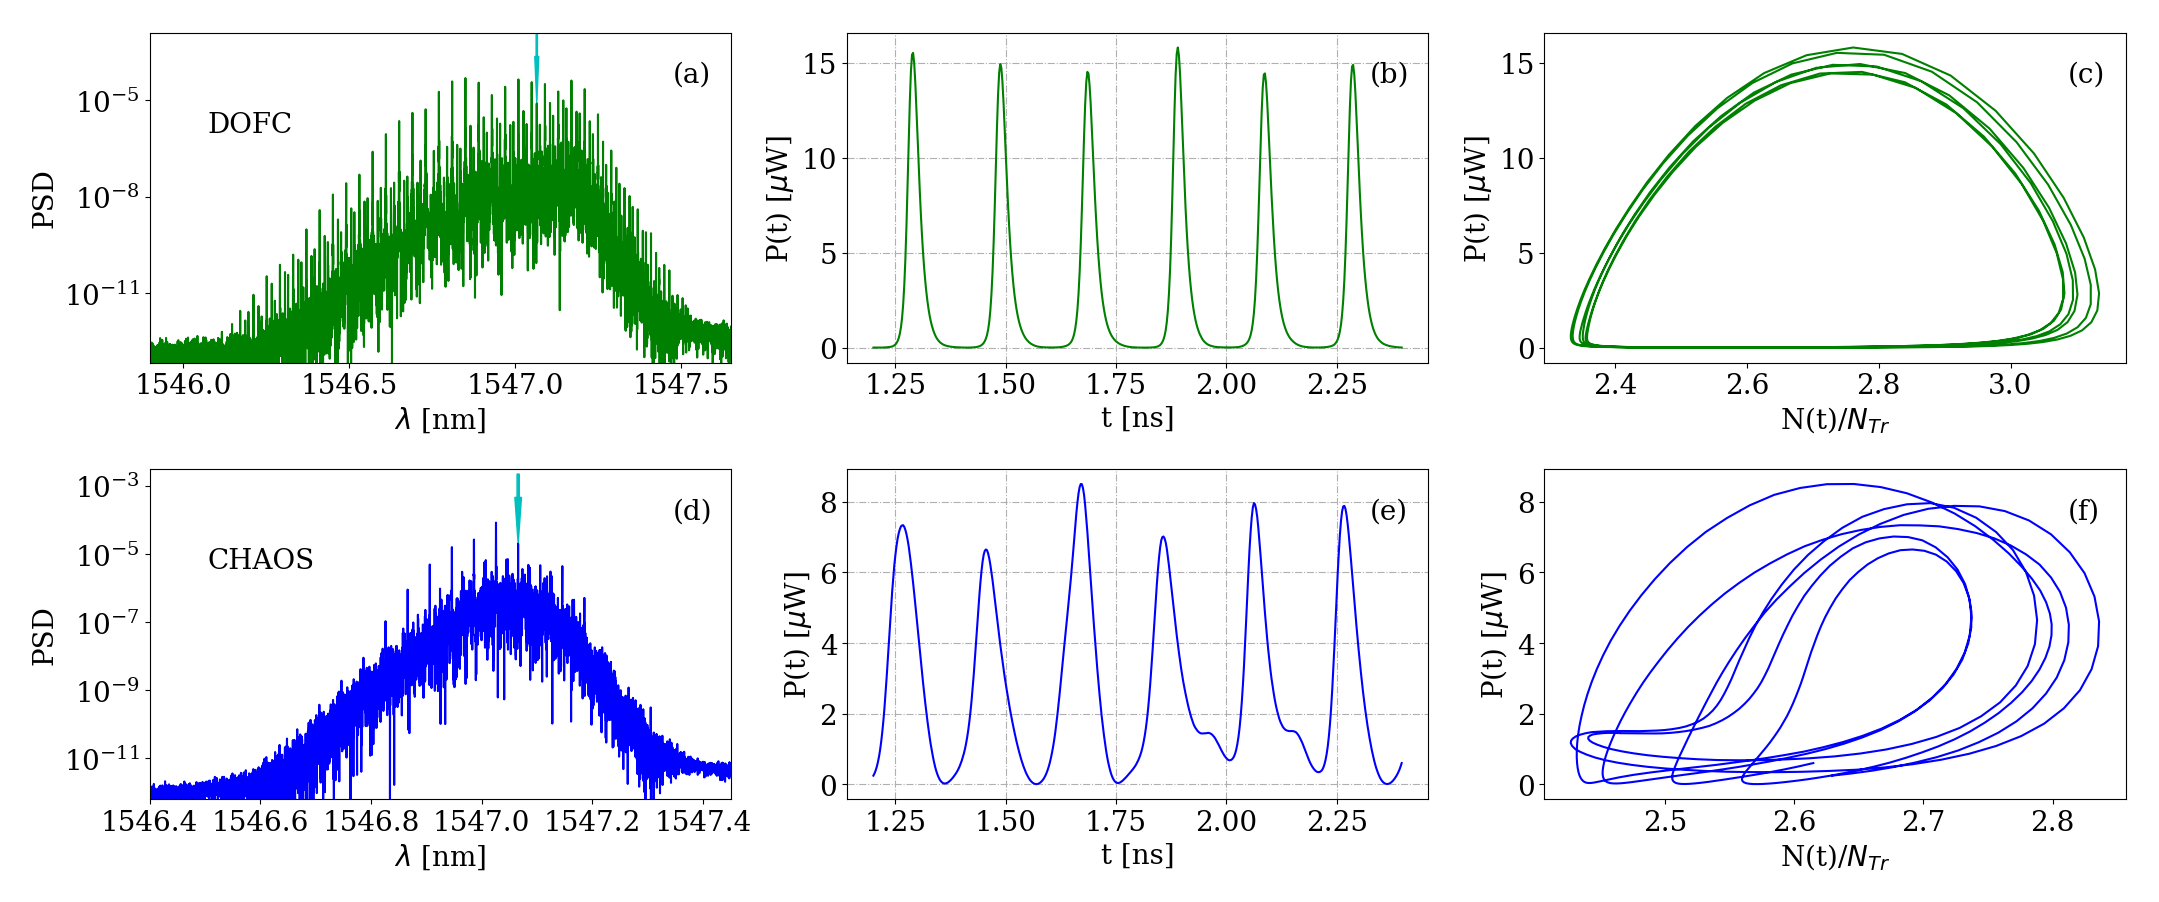
\includegraphics[width=1.0\linewidth]{chaos.png}
				\caption{\label{fig:chaos}Espectros \'opticos, $P(t)$ y atractor en el espacio de los estados de las ecuaciones de balance, despreciando los efectos de la fase \'optica; para $\delta\nu = -2$GHz y $P_{Iny} = 1\;\mu$W (DOFC, naranja) y $300\;\mu$W (CHAOS, azul).}	
			\end{figure}

		El espectro \'optico del DOFC (Figura \ref{fig:chaos} (a)) permite observar varias l\'ineas de emisión bien resultas y con una anchura entre ellas pequeña y bien definida. Ambos espectros \'opticos presentan un perfil similar formado por una ancha banda de ruido debido a la emisi\'on espont\'anea y l\'ineas de emisión que emergen de \'esta. Para el caso de CHAOS estos picos de emisi\'on son mucho menores que para el DOFC. La diferencia entre ambas regiones se hace m\'as notoria en la potencia $P(t)$, en la que para el caso del CHAOS (Figura \ref{fig:chaos} (e)) se observan oscilaciones con diferentes amplitudes para cada pido y diferentes tiempos entre \'estos. Los atractores obtenidos no dejan ninguna duda a la diferncia entre ambas regiones, obteniendo un diagrama tipo caos para $P_{Iny} = 300\;\mu$W en el que se tiende a tomar valores entodo el espacio de estados. Para el caso del DOFC se obtiene un diagrama de tipo P1 (Figura \ref{fig:chaos} (c) pero con algunas diferencias en los trazos.

%
				%\cite{rosado2018experimental}
%
			\addtocontents{toc}{\vspace{0.1cm}}
			\chapter{Conclusiones}

				hola a todos

		%----------------------------------------------------------------------------------------
		%     BIBLIOGRAPHY
		%----------------------------------------------------------------------------------------

			\bibliographystyle{unsrt}
			\bibliography{biblio}

		%----------------------------------------------------------------------------------------
		%     APPENDIX
		%----------------------------------------------------------------------------------------
				
			\newpage

				\appendix

					\chapter{Código de la simulación}

						\definecolor{gray97}{gray}{.97}
\definecolor{gray75}{gray}{.75}
\definecolor{gray45}{gray}{.45}

\lstset{ frame=Ltb,
	framerule=0pt,
	aboveskip=0.1cm,
	framextopmargin=3pt,
	framexbottommargin=3pt,
	framexleftmargin=0.4cm,
	framesep=0pt,
	rulesep=.4pt,
	backgroundcolor=\color{gray97},
	rulesepcolor=\color{black},
	%
	stringstyle=\ttfamily,
	showstringspaces = false,
	basicstyle=\small\ttfamily,
	commentstyle=\color{gray45},
	keywordstyle=\bfseries,
	%
	numbers=left,
	numbersep=15pt,
	numberstyle=\tiny,
	numberfirstline = false,
	breaklines=true,
}

\lstdefinestyle{Python}
{basicstyle=\scriptsize\bf\ttfamily,
language=python,
}

\centering\small
\vspace{0.4cm} +- - - - - - - - - - - - - 18 l\'ineas - - - - - - - - - - - - -+
\lstinputlisting[style=Python, firstline=19, lastline=26, firstnumber=19]{../src/simulation.py}
\vspace{-0.4cm} +- - - - - - - - - - - - - 18 l\'ineas - - - - - - - - - - - - -+
\lstinputlisting[style=Python, firstline=44, lastline=53, firstnumber=44]{../src/simulation.py}

\vspace{-0.4cm} +- - - - - - - - - - - - - 24 l\'ineas - - - - - - - - - - - - -+
\lstinputlisting[style=Python, firstline=77, lastline=81, firstnumber=77]{../src/simulation.py}

\vspace{-0.4cm} +- - - - - - - - - - - - - 15 l\'ineas - - - - - - - - - - - - -+
\lstinputlisting[style=Python, firstline=96, lastline=96, firstnumber=96]{../src/simulation.py}

\vspace{-0.4cm} +- - - - - - - - - - - - - 20 l\'ineas - - - - - - - - - - - - -+
\newpage
\lstinputlisting[style=Python, firstline=116, lastline=155, firstnumber=116]{../src/simulation.py}

\vspace{-0.4cm} +- - - - - - - - - - - - - 10 l\'ineas - - - - - - - - - - - - -+
\newpage
\lstinputlisting[style=Python, firstline=165, lastline=192, firstnumber=165]{../src/simulation.py}

\vspace{-0.4cm} +- - - - - - - - - - - - - 10 l\'ineas - - - - - - - - - - - - -+
\lstinputlisting[style=Python, firstline=202, lastline=206, firstnumber=202]{../src/simulation.py}

\vspace{-0.4cm} +- - - - - - - - - - - - -  6 l\'ineas - - - - - - - - - - - - -+
\lstinputlisting[style=Python, firstline=212, lastline=220, firstnumber=212]{../src/simulation.py}

\vspace{-0.4cm} +- - - - - - - - - - - - - 39 l\'ineas - - - - - - - - - - - - -+
%\lstinputlisting[style=Python, firstline=96, lastline=220, firstnumber=100]{../src/simulation.py}


	\end{document}

%----------------------------------------------------------------------------------------
%              END
%----------------------------------------------------------------------------------------
